\documentclass[twoside,11pt]{article}

% Any additional packages needed should be included after jmlr2e.
% Note that jmlr2e.sty includes epsfig, amssymb, natbib and graphicx,
% and defines many common macros, such as 'proof' and 'example'.
%
% It also sets the bibliographystyle to plainnat; for more information on
% natbib citation styles, see the natbib documentation, a copy of which
% is archived at http://www.jmlr.org/format/natbib.pdf

%\usepackage{jmlr2e}

% my added packages: copied from the swiss IJ paper
\usepackage{microtype}
\usepackage{graphicx}
\usepackage{subfigure}
\usepackage{booktabs} % for professional tables
\usepackage{siunitx}
\usepackage{hyperref}
\usepackage{xargs}[2008/03/08]

% Documentation
% http://ftp.math.purdue.edu/mirrors/ctan.org/macros/latex/contrib/refstyle/refstyle.pdf
\usepackage{refstyle}
\usepackage{varioref} % Use refstyle instead of varioref directly.
\usepackage[authoryear]{natbib}

% \usepackage{prettyref}
% \usepackage{refstyle}

\usepackage{amsmath}
\usepackage{amssymb}
\usepackage{amsfonts}
\usepackage{amsthm}
\usepackage{mathrsfs}
\usepackage{mathtools}
\usepackage{colonequals}
\usepackage{algpseudocode, algorithm} %typical alg typesetting packages

\usepackage{listings}
\usepackage{pdfpages}

% This picks up the knitr boilerplate, allowing us to \input partial knitr
% documents.
\usepackage[]{graphicx}
\usepackage[]{color}
%% maxwidth is the original width if it is less than linewidth
%% otherwise use linewidth (to make sure the graphics do not exceed the margin)
\makeatletter
\def\maxwidth{ %
  \ifdim\Gin@nat@width>\linewidth
    \linewidth
  \else
    \Gin@nat@width
  \fi
}
\makeatother

\definecolor{fgcolor}{rgb}{0.345, 0.345, 0.345}
\newcommand{\hlnum}[1]{\textcolor[rgb]{0.686,0.059,0.569}{#1}}%
\newcommand{\hlstr}[1]{\textcolor[rgb]{0.192,0.494,0.8}{#1}}%
\newcommand{\hlcom}[1]{\textcolor[rgb]{0.678,0.584,0.686}{\textit{#1}}}%
\newcommand{\hlopt}[1]{\textcolor[rgb]{0,0,0}{#1}}%
\newcommand{\hlstd}[1]{\textcolor[rgb]{0.345,0.345,0.345}{#1}}%
\newcommand{\hlkwa}[1]{\textcolor[rgb]{0.161,0.373,0.58}{\textbf{#1}}}%
\newcommand{\hlkwb}[1]{\textcolor[rgb]{0.69,0.353,0.396}{#1}}%
\newcommand{\hlkwc}[1]{\textcolor[rgb]{0.333,0.667,0.333}{#1}}%
\newcommand{\hlkwd}[1]{\textcolor[rgb]{0.737,0.353,0.396}{\textbf{#1}}}%
\let\hlipl\hlkwb

\usepackage{framed}
\makeatletter
\newenvironment{kframe}{%
 \def\at@end@of@kframe{}%
 \ifinner\ifhmode%
  \def\at@end@of@kframe{\end{minipage}}%
  \begin{minipage}{\columnwidth}%
 \fi\fi%
 \def\FrameCommand##1{\hskip\@totalleftmargin \hskip-\fboxsep
 \colorbox{shadecolor}{##1}\hskip-\fboxsep
     % There is no \\@totalrightmargin, so:
     \hskip-\linewidth \hskip-\@totalleftmargin \hskip\columnwidth}%
 \MakeFramed {\advance\hsize-\width
   \@totalleftmargin\z@ \linewidth\hsize
   \@setminipage}}%
 {\par\unskip\endMakeFramed%
 \at@end@of@kframe}
\makeatother

\definecolor{shadecolor}{rgb}{.97, .97, .97}
\definecolor{messagecolor}{rgb}{0, 0, 0}
\definecolor{warningcolor}{rgb}{1, 0, 1}
\definecolor{errorcolor}{rgb}{1, 0, 0}
\newenvironment{knitrout}{}{} % an empty environment to be redefined in TeX

\usepackage{alltt}


% This defines math macros.

% Operators
\def\mbe{\mathbb{E}}%
\def\ind#1{\mathbb{I}\left(#1\right)}
\def\evalat#1#2{\left.#1\right|_{#2}}
\def\fracat#1#2#3{\left.\frac{#1}{#2}\right\vert_{#3}}
\def\iid{\overset{iid}{\sim}}
\def\expect#1#2{\underset{#1}{\mathbb{E}}\left[#2\right]}
\def\cov#1#2{\underset{#1}{\mathrm{Cov}}\left(#2\right)}
\def\expecthat#1#2{\underset{#1}{\widehat{\mathbb{E}}}\left[#2\right]}
\def\abs#1{\left|#1\right|}
\def\norm#1{\left\Vert#1\right\Vert}
\def\norminf#1{\left\Vert#1\right\Vert_{\infty}}
\def\sumk{\sum_{\k=1}^{\kmax}}
\def\sumkm{\sum_{\k=1}^{\kmax - 1}}
\def\dirderiv#1#2{\delta_{#1\rightarrow#2}} % A directional derivative (unused?)
\def\linop{\mathcal{L}} % A linear operator

\DeclareMathOperator*{\argmax}{\mathrm{argmax}}
\DeclareMathOperator*{\argmin}{\mathrm{argmin}}
\DeclareMathOperator*{\esssup}{\mathrm{esssup}}

% Variables
\def\etaopt{\hat\eta} % Optimal vb parameters
\def\x{x}   % Data
\def\t{t}   % Generic priur parameter
\def\z{z}   % Cluster indicators
\def\g{g}   % Function of interest
\def\k{k}   % Cluster index
\def\n{n}   % Data index
\def\nuk{\nu_{\k}}   % K-th stick.  Have to type this a lot.
\def\const{C}   % Constant
\def\lnu{\tilde{\nu}}   % Unconstrained stick
\def\lnumean{\eta^{\mu}}   % Unconstrained stick vb mean
\def\lnusd{\eta^{\sigma}}   % Unconstrained stick vb std
\def\hess#1{H_{#1}}   % Hessian
\def\phiz{0_\phi}   % The phi zero function.
\def\infl{\psi}   % The influence function
\def\inflg{\psi_{\g}}   % The influence function for a function of interest

\def\etatheta{\eta_{\theta}}  % VB parameters for certain components
\def\etanu{\eta_{\nu}}  % VB parameters for certain components
\def\etanuk{\eta_{\nuk}}  % VB parameters for certain components
\def\etaz{\eta_{\z}}  % VB parameters for certain components
\def\etaglob{\eta_{\gamma}}  % VB parameters for theta and nu
\def\etaopttheta{\etaopt_{\theta}}  % VB parameters for certain components
\def\etaoptnu{\etaopt_{\nu}}  % VB parameters for certain components
\def\etaoptnuk{\etaopt_{\nuk}}  % VB parameters for certain components
\def\etaoptz{\etaopt_{\z}}  % VB parameters for certain components
\def\etaoptgamma{\etaopt_{\gamma}}  % VB parameters for certain components


% Distributions
\def\pstick{p_{\mathrm{stick}}}   % Stick breaking distribution
\def\q{q}   % VB dist
\def\logp{\ell}   % Log probabiltty
\def\lqgrad#1{{\nabla \log \q}\left(#1\right)}   % Log VB distribution gradient
\def\lqhess#1{{\nabla^2 \log \q}\left(#1\right)}   % Log VB distribution Hessian
\def\lqgradbar#1{\overline{\lqgrad{#1}}\,\,}   % Log VB distribution gradient centered
\def\lqhessbar#1{\overline{\lqhess{#1}}\,\,}   % Log VB distribution Hessian centered
\def\normdist#1{\mathcal{N}\left(#1\right)}   % Normal distribution
\def\KL#1{\mathrm{KL}\left(#1\right)}   % KL divergence
\def\KLgrad#1{\mathrm{KL}_{\eta}\left(#1\right)}   % KL divergence
\def\KLhess#1{\mathrm{KL}_{\eta\eta}\left(#1\right)}   % KL divergence
\def\wishart#1{\mathrm{Wishart}\left(#1\right)}   % Wishart distribution
\def\gammadist#1{\mathrm{Gamma}\left(#1\right)}   % Gamma distribution
\def\betadist#1{\mathrm{Beta}\left(#1\right)}   % Gamma distribution
\def\pb{p_{0}}   % Base prior
\def\pa{p_{1}}   % Alternative prior

% Taylor series
\def\etalin{\etaopt^{\mathrm{lin}}}
\def\glin{\g^{\mathrm{lin}}}
\def\gapprox{\g^{\etalin}}

% Dimensions
\def\N{N}   % Number of datapoints
\def\K{K}   % Number of components
\def\kmax{{\K_{\mathrm{max}}}}   % Truncation
\def\etadim{{D_{\eta}}}
\def\thetadim{{D_{\theta}}}
\def\zetadim{{D_{\zeta}}}
\def\ngh{N_{\mathrm{GH}}}   % Number of GH points

% Domains
\def\etadom{\Omega_{\eta}}
\def\thetadom{\Omega_{\theta}}
\def\tdom{\Omega_{\t}}
\def\linf{{L_{\infty}[0,1]}}
\def\ball{\mathcal{B}}

% Annotations
\def\mathtxt#1{\quad\textrm{#1}\quad}%
\def\mathand{\quad\textrm{and}\quad}%
\def\mathwhere{\quad\textrm{where}\quad}%
\def\constdesc#1{\textrm{(}\const\textrm{ does not depend on }#1\textrm{)}}
\def\assuitemref#1#2{\assuref{#1} (\itemref{#2})}%


% This specifies the formatting for references (sections, theorems, etc.)

%%%%%%%%%%%%%%%%%%%%
% amsthm commands

\theoremstyle{plain}
\newtheorem{lem}{Lemma}
\newtheorem{thm}{Theorem}
\newtheorem{prop}{Proposition}
\newtheorem{cond}{Condition}
\newtheorem{assu}{Assumption}
\newtheorem{cor}{Corollary}
\newtheorem{conj}{Conjecture}

%\theoremstyle{definition}
% \newtheorem{defn}{Definition}
%\newtheorem{ex}{Example}

% Example environment with a terminating symbol.
% https://tex.stackexchange.com/questions/16453/denoting-the-end-of-example-remark
\theoremstyle{definition}
\newtheorem{examplex}{Example}
\newenvironment{ex}
  {\pushQED{\qed}\renewcommand{\qedsymbol}{$\triangle$}\examplex}
  {\popQED\endexamplex}

\theoremstyle{definition}
\newtheorem{defnx}{Definition}
\newenvironment{defn}
    {\pushQED{\qed}\renewcommand{\qedsymbol}{$\boxdot$}\defnx}
    {\popQED\enddefnx}


\newcommand{\seeproof}[1]{(See \proofref{#1} \proofpageref[vref]{#1}.)}
\newcommand{\proofof}[1]{\noindent{\bf Proof of #1.}}


%%%%%%%%%%%%%%%%%%%%
% refstyle commands

\newref{event}{
    name=Event~, %
    names=Events~, %
    Name=Event~,
    Names=Events~
    }

\newref{item}{
    name=Item~, %
    names=Items~, %
    Name=Item~,
    Names=Items~
    }

\newref{fig}{
    name=Figure~, %
    Name=Figure~
    }

\newref{tab}{
    name=Table~, %
    Name=Table~
    }

\newref{sec}{
    name=Section~, %
    Name=Section~,
    names=Sections~,
    Names=Sections~,
    }

\newref{app}{
    name=Appendix~, %
    Name=Appendix~
    }

\newref{eq}{
    name=Eq.~, %
    Name=Eq.~,
    names=Eqs.~, %
    Names=Eqs.~
    }

\newref{fig}{
    name=Figure~, %
    Name=Figure~,
    names=Figures~, %
    Names=Figures~,
    }

\newref{def}{
    name=Definition~, %
    Name=Definition~
    }

\newref{assu}{
    name=Assumption~, %
    Name=Assumption~,
    names=Assumptions~, %
    Names=Assumptions~,
    }

\newref{cond}{
    name=Condition~, %
    Name=Condition~,
    names=Conditions~, %
    Names=Conditions~
    }

\newref{prop}{
    name=Proposition~, %
    Name=Proposition~,
    names=Propositions~, %
    Names=Propositions~
    }

\newref{lem}{
    name=Lemma~, %
    Name=Lemma~,
    names=Lemmas~, %
    Names=Lemmas~
    }

\newref{ex}{
    name=Example~, %
    Name=Example~,
    names=Examples~,
    Names=Examples
    }

\newref{cory}{
    name=Corollary~, %
    Name=Corollary~
    }

\newref{thm}{
    name=Theorem~, %
    Name=Theorem~,
    names=Theorems~, %
    Names=Theorems~
    }

\newref{proof}{
    name=Proof~, %
    Name=Proof~
    }

\newref{conj}{
    name=Conjecture~, %
    Name=Conjecture~
    }

\newref{algr}{
    name=Algorithm~, %
    Name=Algorithm~,
    names=Algorithms~, %
    Names=Algorithms~,
    }


%% refstyle examples:
% \Secref[vref]{introduction} contains \secref{introduction}.
% \Secref[vref]{ack} does not contain \secref{introduction}.
%
% \begin{align}
%     x=y \eqlabel{myeq}
% \end{align}
%


% Heading arguments are {volume}{year}{pages}{date submitted}{date published}{paper id}{author-full-names}

%\jmlrheading{1}{2000}{1-48}{4/00}{10/00}{giordano21}{Ryan Giordano and Runjing Liu and Michael I. Jordan and Tamara Broderick}

% Short headings should be running head and authors last names

%\ShortHeadings{BNP sensitivity}{Giordano et al.}
%\firstpageno{1}

\begin{document}

\title{Evaluating Sensitivity to the Stick Breaking Prior in Bayesian Nonparametrics}

\author{Ryan Giordano \texttt{rgiordan@mit.edu} \\
        \and
        Runjing Liu \texttt{runjing\_liu@berkeley.edu} \\
        \and
        Michael I.\ Jordan \texttt{jordan@cs.berkeley.edu} \\
        \and
        Tamara Broderick \texttt{tbroderick@csail.mit.edu }
        }

\maketitle

\begin{abstract}%   <- trailing '%' for backward compatibility of .sty file
This is an abstract
\end{abstract}

\section{Introduction}\label{sec:introduction}
Scientists, engineers, and social scientists are often interested in inferring
the number of clusters in a given data set, as well as which observations
cluster together. A common methodology builds on the Dirichlet process
\citep{ferguson:1973:bayesian, sethuraman:1994:constructivedp} from Bayesian
nonparametrics (BNP). BNP methods offer a number of favorable properties. They
allow the number of clusters to grow with the size of the data set; for example,
we might expect to keep discovering new species as we examine more individual
organisms, and we might expect to discover more topics as we read more articles
in a scientific journal. Moreover, BNP methods can be flexibly incorporated into
models of varying complexity. And the Dirichlet process in particular offers a
convenient and well-studied prior on the number and assignment of clusters --
facilitating Bayesian posterior inference and a resulting coherent
quantification of uncertainty.

Nonetheless, Bayesian modeling often involves choices of convenience rather than
pure subjective prior elicitation, and Dirichlet process models are no
exception. For instance, the latent frequencies of clusters -- i.e., the
component proportions -- in a Dirichlet process are generated by recursively
removing beta-distributed fractions of probability mass from the unit interval.
The beta distribution is historically convenient for approximate inference
methods (such as Gibbs sampling) that rely on conditional conjugacy but need not
represent a strong prior belief. Similarly, the Dirichlet process concentration
parameter $\alpha$ may often be chosen based on previous applications rather
than prior belief for the application at hand.
\todo{Cite something (Ryan doesn't have ideas.)}

In general, then, there often exist many possible $\alpha$ values, and many
possible forms of stick-breaking, that might correspond to our prior beliefs.
And these choices can change the results of a data analysis. For instance,
$\alpha$ asymptotically serves as a proportionality constant for the number of
clusters. So the number of clusters at any particular data size may depend
strongly on $\alpha$. If our scientific conclusions varied substantially over
seemingly equivalent prior choices, we might worry that these conclusions are
driven not by our data and meaningful prior beliefs but instead by
somewhat-arbitrary aspects of implementation. It behooves us, then, to check how
sensitive our conclusions are to these choices.

In practice, Bayesian inference requires not just specification of a model and
collection of data but also the use of some posterior approximation. So when we
assess the sensitivity of our conclusions, we should assess the sensitivity of
the full procedure we use in practice. Variational Bayes (VB) is a particularly
popular posterior approximation method for unsupervised learning problems such
as clustering and topic modeling due its fast computation time, increasingly
automated implementations \citep{ranganath:2013:black, kucukelbir:2016:advi},
and avoidance of the label-switching problem exhibited by MCMC
\citep{jasra:2005:mcmclabelswitch}. Therefore, we imagine in what follows that
we have computed the VB approximation for some clustering quantity of interest,
such as number of clusters or cluster co-occurrence.

With a full methodology for clustering in hand, we now can ask how sensitive our
quantity of interest is to the choices of $\alpha$ and the stick-breaking
distributions. One option is to propose a number of potential $\alpha$ values,
compute the variational approximation at each $\alpha$ value, and report our
quantity of interest for each $\alpha$ value. We might similarly assess
sensitivity to the stick-breaking distribution over a range of distributional
choices. There are at least two major issues with this proposal: (1) while VB is
a relatively fast form of approximation Bayesian inference in general, it may
still be prohibitively expensive to have to re-run it many times and (2) it is
unclear how best to choose a collection of $\alpha$ and (especially) the
stick-breaking distribution values -- and how many to choose.

In this work, we circumvent these challenges with a local approximation. VB
posits posterior approximation as an optimization problem. So we show how to
approximate the nonlinear dependence of the VB optimum on prior choices using a
first-order Taylor series expansion. We build on the local robustness tools
developed by \cite{giordano:2018:covariances} for VB and
\cite{gustafson:1996:local} for MCMC. To enable their application to VB for BNP
clustering, we solve a number of open problems; indeed the techniques we
introduce in the current work may be seen to advance sensitivity for VB more
broadly. (1) In particular, we establish that the optimal VB parameters are a
continuously differentiable function of $\alpha$ and the stick-breaking form.
(2) We show that the sensitivity of the VB approximation to functional prior
perturbations takes the form of an integral against a computationally tractable
\textit{influence function} -- and illustrate how the influence function can
provide an interpretable summary of the effect of arbitrary changes to the prior
density. (3) To justify using linear approximations over a ball describing
different stick-breaking densities, we show that our approximation is
\textit{uniformly} good by establishing Fr\'echet differentiability. (4) We how
to efficiently compute our approximation even in high-dimensional problems,
e.g.\ as arise in BNP models. (5) We establish the accuracy, practicality, and
speed of our approximation for a variety of models that use stick-breaking, and
for various quantities of interest in both clustering and topic modeling.



\section{Stick-breaking Dirichlet processes}


\section{Local sensitivity}
Consider the optimization problem \eqref{vb_optimization}, but now let the
priors $\pstick(\nuk)$ which enter the term $\logp(\zeta)$ depend on a
real-valued parameter, $\t \in \tdom \subseteq \mathbb{R}$, writing
$\pstick(\nuk \vert \t)$.

%%%%%%%%%%%%%%%%%%%%%%%%%%%%%%%%%%%%%%%%%%%%%%%%%%%%%%%%%%%%%%%%%%%%%%%%%%%%%%%%
%%%%%%%%%%%%%%%%%%%%%%%%%%%%%%%%%%%%%%%%%%%%%%%%%%%%%%%%%%%%%%%%%%%%%%%%%%%%%%%%
\begin{ex}\exlabel{alpha_perturbation}
%
When drawing from the classical $\mathrm{GEM}(\alpha)$ distribution, we
model
%
\begin{align*}
%
\pstick(\nuk \vert \alpha) ={}&
    \betadist{\nuk \vert 1, \alpha} \Rightarrow\\
\log \pstick(\nuk \vert \alpha) ={}&
    (\alpha - 1) \log(1 - \nuk) + \const. &
    \constdesc{\nuk}
%
\end{align*}
%
Fix some ``original'' $\alpha_0$.  In this case, we represent deviations from the
choice $\alpha_0$ by identifying $\t$ with $\alpha - \alpha_0$:
%
\begin{align}\eqlabel{gem_alpha_pert}
%
\log \pstick(\nuk \vert \alpha) ={}&
    (\alpha + \alpha_0 - 1) \log(1 - \nuk) + \const.
    %& \constdesc{\nuk}
%
\end{align}
%
\end{ex}
%%%%%%%%%%%%%%%%%%%%%%%%%%%%%%%%%%%%%%%%%%%%%%%%%%%%%%%%%%%%%%%%%%%%%%%%%%%%%%%%

In \secref{prior_perturbations}, we will consider a more general class of
perturbations than \exref{alpha_perturbation}.

In any case, the prior on $\zeta$ and posterior in turn depend on $\t$, which we
write $\p(\zeta \vert \x, \t)$. The $\t$ dependence propagates to the optimal
variational parameters as well through the dependence of the KL divergence on
$\t$.  Define the shorthand notation
%
\begin{align}\eqlabel{kl_shorthand}
%
\KL{\eta, \t} := \KL{\q(\zeta \vert \eta) || \p(\x \vert \zeta, \t)}
\mathand
\etaopt(\t) := \argmin_{\zeta \in \etadom} \KL{\eta, \t},
%
\end{align}
%
where we write $\etaopt(\t)$ to emphasize the dependence of the optimum on $\t$.
Without loss of generality, we will continue to use $\etaopt$ with no argument
to refer to $\etaopt(0)$.  That is, we take $\t = 0$ at the ``original''
problem, \eqref{vb_optimization}.

If the map $\t \mapsto \etaopt(\t)$ is continuously differentiable, and we have
already computed the solution $\etaopt$ to the ``original'' problem
\eqref{vb_optimization}, then we can form a Taylor series approximation to
$\etaopt(\t)$.  Specifically, we define
%
\begin{align}\eqlabel{etalin_def}
%
\etalin(\t) := \etaopt + \fracat{d \etaopt(\t)}{d \t}{\t=0} \t .
%
\end{align}
%
Evaluating $\etaopt(\t)$ requires solving a new optimization problem, but, given
$d\etaopt(\t) / d\t | 0$, evaluating $\etalin(\t)$ involves only
multiplication and addition.  When $|\t|$ is small, by continuous
differentiability of $\etaopt(\t)$, we might hope that $\etaopt(\t) \approx
\etalin(\t)$, and so we can use $\etalin(\t)$ to quickly approximate a
time-consuming optimization problem.

Futhermore, or functions of interest $\g(\eta)$ which are themselves
differentiable, we can use the chain rule to compute
%
\begin{align}\eqlabel{vb_g_sens}
%
\fracat{d g(\etaopt(\t))}{d\t} ={}&
    \fracat{\partial g(\eta)}{\partial \eta^T}{\etaopt(\t_0)}
    \fracat{d \etaopt(\t)}{d \t}{\t_0} \\
\glin(\t) :={}& \g(\etaopt(\t_0)) + \fracat{d g(\etaopt(\t))}{d\t}{\t_0} (\t - \t_0).
%
\end{align}
%
For non-differentiable functions of $\eta$, we can still form the approximation
%
\begin{align*}
%
\gapprox(\t) :={}& \g(\etalin(\t)).
%
\end{align*}
%
The advantage of $\glin(\t)$ relative to $\gapprox(\t)$ is that for the former
we can compute influence functions and worst-case perturbations, as we discuss
below in \secref{prior_perturbations}.  Converse, $\gapprox(\t)$ may be expected
to provide a better approximation in some cases since it retains non-linearities
in the map $\eta \mapsto \g(\eta)$, linearizing only the computationally
intensive map $\t \mapsto \etaopt(\t)$.

When, then, is $\etaopt(\t)$ continuously differentiable?  We now state some
sufficient conditions which will allow us to prove that $\etaopt(\t)$ is
continuously differentiable via the implicit function theorem
(e.g., \citet{krantz:2012:implicit}).


%%%%%%%%%%%%%%%%%%%%%%%%%%%%%%%%%%%%%%%%%%%%%%%%%%%%%%%%%%%%%%%%%%%%%%%%%%%%
%%%%%%%%%%%%%%%%%%%%%%%%%%%%%%%%%%%%%%%%%%%%%%%%%%%%%%%%%%%%%%%%%%%%%%%%%%%%
\begin{assu}\assulabel{dist_fun_nice}
%
TODO: I think you might need to be more careful about the uniformity
in $\eta$.  In particular, does the bound need to hold for any particular
$\eta$, or does the supremum of bounds over $\eta$ need to be finite?

Let $\q(\theta \vert \eta)$ be a (possibly unnormalized) density over the random
variable $\theta$ parameterized by $\eta$ defined relative to a dominating
measure $\lambda$.  Assume that the map $\eta \mapsto \log \q(\theta \vert
\eta)$ is twice continuously differentiable.

Let $\psi(\theta, \t)$ be a scalar-valued $\lambda$-measurable function of
$\theta$ and $\t$.  Assume that the map $\t \mapsto \psi(\theta, \t)$ is
continuously differentiable.

Define the following shorthand notation:
%
\begin{align*}
%
\lqgrad{\theta \vert \eta} :={}&
    \fracat{\partial \log \q(\theta \vert \eta)}{\partial \eta}{\eta} \\
%
\lqhess{\theta \vert \eta} :={}&
    \fracat{\partial^2 \log \q(\theta \vert \eta)}
           {\partial \eta \partial \eta^T}{\eta} \\
%
\psigrad{\theta, \t} :={}& \fracat{\partial \psi(\theta, \t)}{\partial \t}{\t}.
%
\end{align*}
%
For a given $\t_0$ and $\eta_0$, assume there exists some neighborhood of
$\t_0$, $\ball_\t$, some neighborhood of $\eta_0$, $\ball_\eta$, and a
$\lambda$-integrable $M_\psi(\theta)$ with $\int M_\psi(\theta) \lambda(d\theta) <
\infty$ such that the following bounds hold for all $\eta, \t \in \ball_\eta
\times \ball_\t$:
%
\begin{enumerate}
%
\item \itemlabel{fundom}
$\q(\theta \vert \eta) \psi(\theta, \t) \le M_\psi(\theta)$.
%
\item \itemlabel{funqgraddom}
$\q(\theta \vert \eta) \norm{\lqgrad{\theta \vert \eta}}_2 \psi(\theta, \t) \le
M_\psi(\theta)$.
%
\item \itemlabel{funqhessdom}
$\q(\theta \vert \eta) \norm{\lqhess{\theta \vert \eta}}_2 \psi(\theta, \t) \le
M_\psi(\theta)$.
%
\item \itemlabel{fungradqgraddom}
$\q(\theta \vert \eta) \norm{\lqgrad{\theta \vert \eta}}_2 \psigrad{\theta, \t}
\le M_\psi(\theta)$.
%
\item \itemlabel{funqgradsqdom}
$\q(\theta \vert \eta) \norm{\lqgrad{\theta \vert \eta}}^2_2 \psi(\theta, \t) \le
M_\psi(\theta)$.
%
\end{enumerate}
%
\end{assu}
%%%%%%%%%%%%%%%%%%%%%%%%%%%%%%%%%%%%%%%%%%%%%%%%%%%%%%%%%%%%%%%%%%%%%%%%%%%%

\Assuref{dist_fun_nice} states sufficient conditions for which we can apply the
dominated convergence theorem to varaiational expectations, allowing us to
translate continuity of the variational and model densitites into continuity of
the variational objective.  The details can be found in \lemref{logq_derivs,
logq_continuous} of \appref{cont_lemmas}.  We might equivalently have said that
we can exchange limits and variational expectations whenever needed,
\assuref{dist_fun_nice} simply being a precise catalogue of what is needed.


%%%%%%%%%%%%%%%%%%%%%%%%%%%%%%%%%%%%%%%%%%%%%%%%%%%%%%%%%%%%%%%%%%%%%%%%%%%%
%%%%%%%%%%%%%%%%%%%%%%%%%%%%%%%%%%%%%%%%%%%%%%%%%%%%%%%%%%%%%%%%%%%%%%%%%%%%
\begin{assu}\assulabel{kl_opt_ok}
%
Let the following conditions on the variational approximation hold.
%
%%%%%%%%%%%%%%%%%%%%%%%%%%%%%%%%%%%%%%%%%%%%%%%%%%%%%%%%%%%%%%%%%%%%%%
\begin{enumerate}
%
    \item \itemlabel{kl_opt_interior} The optimal $\etaopt$ is interior
    to $\etadom$.

    \item \itemlabel{kl_diffable} The map $\eta \mapsto \KL{\eta, 0}$ is twice
    continuously differentiable at $\etaopt$.

    \item\itemlabel{kl_hess} The Hessian matrix $\fracat{\partial^2 \KL{\eta,
    0}} {\partial \eta \partial \eta^T} {\etaopt}$ is positive definite.
%
\end{enumerate}
%
\end{assu}
%%%%%%%%%%%%%%%%%%%%%%%%%%%%%%%%%%%%%%%%%%%%%%%%%%%%%%%%%%%%%%%%%%%%%%%%%%%%

%%%%%%%%%%%%%%%%%%%%%%%%%%%%%%%%%%%%%%%%%%%%%%%%%%%%%%%%%%%%%%%%%%%%%%%%%%%%
%%%%%%%%%%%%%%%%%%%%%%%%%%%%%%%%%%%%%%%%%%%%%%%%%%%%%%%%%%%%%%%%%%%%%%%%%%%%
\begin{assu}\assulabel{q_stick_regular}
%
Assume that the variational approximations $\q(\nu \vert \etanuk)$ to the
stick-breaking posteriors satisfy \assuref{dist_fun_nice} with $\theta = \nuk$,
$\eta_0 = \etaopt$, and with both $\psi(\theta, \t) \equiv 1$ (no $\theta$
dependence) and with $\theta = \nuk$ and $\psi(\nuk, \t) = \log \pstick(\nuk
\vert \t)$, for all $\k$.
%
\end{assu}
%%%%%%%%%%%%%%%%%%%%%%%%%%%%%%%%%%%%%%%%%%%%%%%%%%%%%%%%%%%%%%%%%%%%%%%%%%%%

%%%%%%%%%%%%%%%%%%%%%%%%%%%%%%%%%%%%%%%%%%%%%%%%%%%%%%%%%%%%%%%%%%%%%%%%%%%%
%%%%%%%%%%%%%%%%%%%%%%%%%%%%%%%%%%%%%%%%%%%%%%%%%%%%%%%%%%%%%%%%%%%%%%%%%%%%
\begin{thm}\thmlabel{etat_deriv}
%
Let \assuref{kl_opt_ok, q_stick_regular} hold.  Then the map $\t \mapsto
\etaopt(\t)$ is continuously differentiable with derivative
%
\begin{align}\eqlabel{vb_eta_sens}
%
\fracat{d \etaopt(\t)}{d \t}{0} ={}&
    - \left( \fracat{\partial^2 \KL{\eta, \t}}
                    {\partial \eta \partial \eta^T}
                    {\etaopt, 0} \right)^{-1}
    \fracat{\partial^2 \KL{\eta, \t}}
           {\partial \eta \partial \t}
           {\etaopt, 0}.
%
\end{align}
%
%%%%%%%%%%%%%%%%%%%%%%%%%%%%%%%%%%%%%%%%%%%%%%%%%%%%%%%%%%%%%%%%%%%%%%%%%%%%
%
\begin{proof}
%
For the duration of the proof, define
%
\begin{align*}
%
\rho(\etanuk, \t) :={}&
    \expect{\q(\nu \vert \etanuk)}
           {\log \pstick(\nu \vert \t) - \log \pstick(\nu \vert 0)}
\mathand\\
\rho_\eta(\etanuk, \t) :={}&
\fracat{\partial \rho(\etanuk, \t)}
       {\partial \etanuk}{\etanuk}.
%
\end{align*}
%
Expanding $\logp(\zeta \vert \t)$ in \eqref{vb_optimization}, we see that
%
\begin{align}
%
\logp(\zeta \vert \t) ={}& \logp(\zeta) +
    \sumkm \left( \log \pstick(\nuk\vert\t) -
                  \log \pstick(\nuk \vert 0) \right) \Rightarrow \nonumber\\
\KL{\eta, \t} ={}&
    \KL{\eta, 0} + \sumkm \rho(\etanuk, \t). \eqlabel{kl_pert}
%
\end{align}
%
We thus see that the optimization objective $\KL{\eta, \t}$ is the original
optimization obejctive, $\KL{\eta, 0}$, plus an additive term depending only on
$\etanu$ and $\t$.

By \lemref{logq_derivs}, $\etanuk \mapsto \rho(\etanuk, \t)$ is continuous, and
by \lemref{logq_continuous} $\etanuk \mapsto \rho(\etanuk, \t)$ is continuously
differentiable, for all $\eta, \t \in \ball$.  So $\partial \KL{\eta, \t}  /
\partial \eta$ is continuous for all $\eta, \t \in \ball$ and, by the
first-order condition of \eqref{kl_shorthand}, $\etaopt(\t)$ satisfies
%
\begin{align}\eqlabel{vb_first_order_condition}
%
\fracat{\partial \KL{\eta, \t}}{ \partial \eta}{\etaopt(\t), \t} ={}
\fracat{\partial \KL{\eta, 0}}{ \partial \eta}{\etaopt(\t)}
+  \sumkm \rho_\eta(\etaoptnuk(\t), \t) ={} 0
%
\end{align}
%
for all $\t \in \ball_\t$.
% Recall that the intractable $\logp(\x \vert \t)$
% does not depend on $\eta$, and so vanishes in \eqref{vb_first_order_condition},
% and in all expressions involving partial $\eta$ derivatives of the KL
% divergence.

We wish to apply the implicit function theorem to
\eqref{vb_first_order_condition}, for which we must show that $\partial
\KL{\eta, \t} / \partial \eta$ is continuously differentiable in both $\eta$ and
$\t$.  By \assuitemref{kl_opt_ok}{kl_diffable}, $\partial \KL{\eta, 0} /
\partial \eta$ is continuously differentiable, so we need only consider
$\rho_\eta(\etanuk, \t)$.

By \lemref{logq_continuous} and \assuref{q_stick_regular}, we
have that both $\partial \rho_\eta(\etanuk, \t) / \partial \eta$ and $\partial
\rho_\eta(\etanuk, \t) / \partial \t$ are continuous in both $\eta$ and $\t$.
Since both its partial derivatives are continuously differentiable, the joint
map $\eta, \t \mapsto \rho_\eta(\eta, \t)$ is also continuously differentiable
(e.g., \citet[Theorem 3.2]{fleming:2012:functions}).  Consequently, $\partial
\KL{\eta, \t} / \partial \eta$ is continuously differentiable in both $\eta$ and
$\t$.

% This does not appear to be necessary.
% Since $\rho_\eta(\eta, \t)$ is continuously differentiable, $\KLhess{\eta, \t}$
% is continuous, and since $\KLhess{\etaopt, 0}$ is positive definite,
% $\KLhess{\eta, \t}$ is positive definite for all $\eta, \t \in \ball$.

Together with \assuitemref{kl_opt_ok}{kl_hess}, which gives that $\partial^2
\KL{\eta, \t} / \partial \eta \partial\eta^T$ is invertible at $\etaopt$, the
result then follows from the implicit function theorem \citet[Theorem
3.3.1]{krantz:2012:implicit}. For convenience, \tabref{kranz_notation} shows the
correspondence between their notation and ours.
% Note
% that we make the following formal identifications with the notation of
% \citet[Theorem 3.3.1]{krantz:2012:implicit}:

\begin{center}
\begin{tabular}{|c|c|}
%
\hline Krantz \& Parks notation & Our notation \\\hline
$\Phi(x)$                       & $\KL{\eta, \t}$ \\\hline
$Q$                             & $1$ \\\hline
$M$                             & $\etadim$ \\\hline
$U$                             & $\ball$ \\\hline
$W$                             & $\ball_\t$ \\\hline
$x_1,\ldots,x_Q$                & $\t$ \\\hline
$x_{Q+1},\ldots,x_N$            & $\eta$ \\\hline
$f_1(x_a), \ldots,f_M(x_a)$     & $\etaopt(\t)$ \\\hline
%Equation 3.32                   & \assuitemref{kl_opt_ok}{kl_hess} \\\hline
%
\end{tabular}\tablabel{kranz_notation}
\end{center}
%
\end{proof}
%
\end{thm}
%%%%%%%%%%%%%%%%%%%%%%%%%%%%%%%%%%%%%%%%%%%%%%%%%%%%%%%%%%%%%%%%%%%%%%%%%%%%

%%%%%%%%%%%%%%%%%%%%%%%%%%%%%%%%%%%%%%%%%%%%%%%%%%%%%%%%%%%%%%%%%%%%%%%%%%%%
%%%%%%%%%%%%%%%%%%%%%%%%%%%%%%%%%%%%%%%%%%%%%%%%%%%%%%%%%%%%%%%%%%%%%%%%%%%%

\begin{cor}\corlabel{our_approximation}
%
For the variational approximation of \secref{model_vb} and perturbation
given in \exref{alpha_perturbation}, $\alpha \mapsto \etaopt(\alpha)$
is continuously differentiable.
%
\end{cor}

%%%%%%%%%%%%%%%%%%%%%%%%%%%%%%%%%%%%%%%%%%%%%%%%%%%%%%%%%%%%%%%%%%%%%%%%%%%%



\section{Results}

\subsection{Gaussian mixture modeling on iris data}
%%%%%%%%%%%%%%%%%%%%%%%%%%%%%%%%%%%%%%
%%%%%%%%%%%%%%%%%%%%%%%%%%%%%%%%%%%%%%
% Do not edit the TeX file your work
% will be overwritten.  Edit the RnW
% file instead.
%%%%%%%%%%%%%%%%%%%%%%%%%%%%%%%%%%%%%%
%%%%%%%%%%%%%%%%%%%%%%%%%%%%%%%%%%%%%%
  


We demonstrate the local sensitivity computations on a 
Gaussian mixture model of the iris dataset. 
The generative model and variational approximation were detailed in 
\exref{iris_bnp_process,iris_var_distr}, respectively. 
\figref{iris_fit} shows the GMM fit at $\alpha = 6$. 
The data consists of three iris species, and
the BNP model correspondingly identifies three dominant clusters. 


\begin{knitrout}
\definecolor{shadecolor}{rgb}{0.969, 0.969, 0.969}\color{fgcolor}\begin{figure}[!h]

{\centering 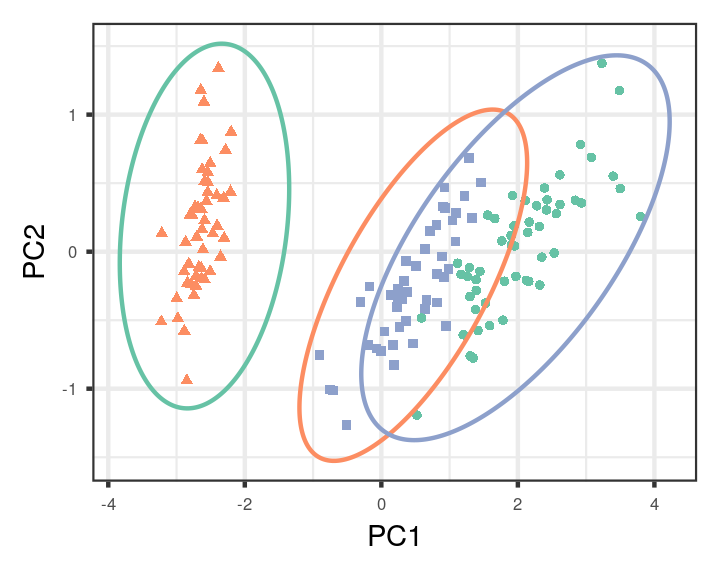
\includegraphics[width=0.588\linewidth,height=0.470\linewidth]{figure/iris_fit-1} 

}

\caption[The iris data in principal component space and 
                      GMM fit at $\alpha = 6$]{The iris data in principal component space and 
                      GMM fit at $\alpha = 6$. 
                      Colors denote inferred memberships and
                      ellipses are estimated covariances. }\label{fig:iris_fit}
\end{figure}


\end{knitrout}

We wish to evaluate the sensitivity of the expected number of clusters to the 
stick-breaking distribution. 
Define the expected number of \textit{in-sample} clusters as
\begin{align*}
\gclusters(\eta) &= \expect{\q(\z\vert\eta)}{\sum_{k=1}^\kmax \ind{ \sum_{n=1}^{N}
\z_{\n\k} > 0}} \\ 
&= \sum_{k=1}^\kmax \left(1 -  \prod_{n=1}^N
\left(1 - \expect{\q(\z_{nk}\vert\eta)}{\z_{nk}}\right)\right).
\end{align*}
The expectation and product can be interchanged because $q$ is mean-field. 

The in-sample quantity $\gclusters$ is an estimate for 
the number of species present in the observed iris dataset. 
Alternatively, we can define a {\itshape posterior predictive} quantity, 
which is an estimate of the number of species one would expect to see 
should a new iris dataset of size $N$ be collected.
Define the posterior predictive number of clusters as 
\begin{align}\eqlabel{post_pred_nclusters}
\gclusterspred(\eta) = \expect{\q(\nu\vert\eta)}{\sum_{k=1}^\kmax\left(1 -
(1 - \pi_k)^N\right)},
\end{align}
where recall that $\pi_k$ are the mixture weights computed from the stick-lengths, $\pi_\k = \nuk \prod_{\k' < \k} (1 - \nu_{\k'})$. 

Unlike the in-sample quantity, the expectation for the predictive quantity is not a simple closed-form function of the variational parameters.  
Instead, we approximate~\eqref{post_pred_nclusters} using Monte Carlo draws from the variational distribution. 
Specifically, we use the ``reparameterization trick" to sample from the variational distribution:
we use an appropriately chosen, $\eta$-dependent transformation 
$f(\cdot, \eta)$ that satisfies 
\begin{align*}
  u \iid\normdist{0, I} \implies 
  f(u, \eta) \stackrel{d}{=} \nu \sim \q(\cdot | \eta).
\end{align*}
To form a Monte Carlo estimate of \eqref{post_pred_nclusters}, 
we sample $u_1, ..., u_m\stackrel{iid}{\sim}\normdist{0, I}$ 
and then average the expression inside the expectation evaluated at points 
$f(u_1, \eta), ..., f(u_m, \eta)$.
We use the reparameterization trick so that conditional on $u_1, ..., u_m$,
our Monte Carlo estimate of $\gclusterspred$ is a determinstic function of 
the variational parameters $\eta$. 
In our experiments below, all displayed values of $\gclusterspred(\eta)$ are
Monte-Carlo approximations, 
conditional on the same $m = 10,000$ draws $u_1, ..., u_m$, fixed a priori. 

We evaluate the sensitivity of the posterior quantities 
$\gclusters$ and $\gclusterspred$ to the prior parameter $\alpha$ in the
$\betadist{\nuk \vert 1, \alpha}$ stick distribution. 
\figref{beta_priors} displays probability density functions of the stick distribution over a range of $\alpha$. 

We fit the initial model at $\alpha = 6$. 
Subsequent refits at $\alpha\not=6$ used the variational parameters at 
$\alpha = 6$ as an initialization. 
As $\alpha$ increases, both the expected in-sample and the expected predictive number of clusters increases (\figref{iris_alpha_sens}). 
The in-sample quantity is relatively insensitive to changes in the $\alpha$ parameter. 
As $\alpha$ varies from $\alpha = 1, ..., 16$, $\gclusters$ varies 
only from 3.0 to 3.4 (recall that the true number of iris species is three). 
On the other hand, the posterior preditive quantity is sensitive 
to changes in $\alpha$.
Over the same range of $\alpha$, $\gclusterspred$ varies from 
3.6 to 8.1. 

We computed the linear approximation at $\alpha = 6$.  
The linear approximation is able to reproduce changes to both 
the in-sample and predictive quantities found by refitting the model at each
$\alpha = 1, ..., 16$ (\figref{iris_alpha_sens}).  
Furthermore, the linear approximation is an order of magnitude faster than refitting. 
Forming the linear approximation, which requires a Hessian inversion (\eqref{vb_eta_sens}), required 0.02 seconds. 
After forming the linear approximation at $\alpha = 6$,
computing $\etalin(\alpha)$ for all $\alpha = 1, ... 16$ took another 
0.02 seconds.
On the other hand, to refit $\etaopt(\alpha)$ for the same range of
$\alpha$'s took a total of 10 seconds, 
with a median refit time of 0.7 seconds. 




\begin{knitrout}
\definecolor{shadecolor}{rgb}{0.969, 0.969, 0.969}\color{fgcolor}\begin{figure}[!h]

{\centering 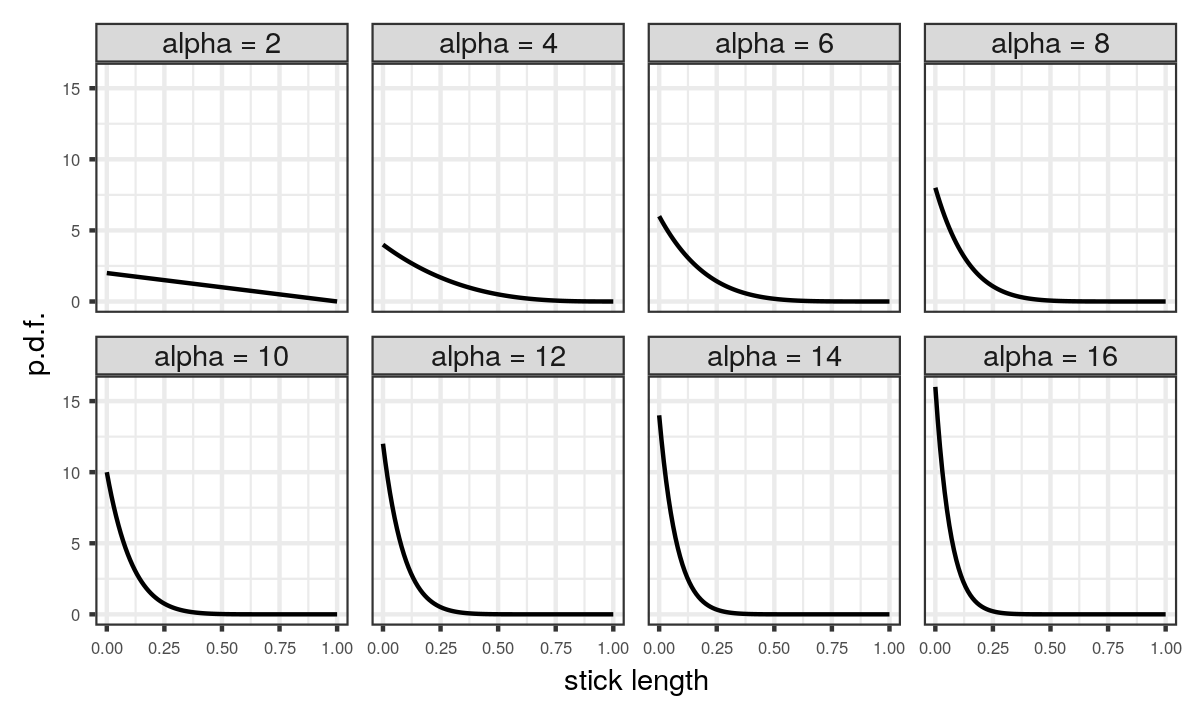
\includegraphics[width=0.980\linewidth,height=0.588\linewidth]{figure/beta_priors-1} 

}

\caption[Probability density functions of $\text{Beta}(1, \alpha)$ distributions, for various $\alpha$]{Probability density functions of $\text{Beta}(1, \alpha)$ distributions, for various $\alpha$. }\label{fig:beta_priors}
\end{figure}


\end{knitrout}




\begin{knitrout}
\definecolor{shadecolor}{rgb}{0.969, 0.969, 0.969}\color{fgcolor}\begin{figure}[!h]

{\centering 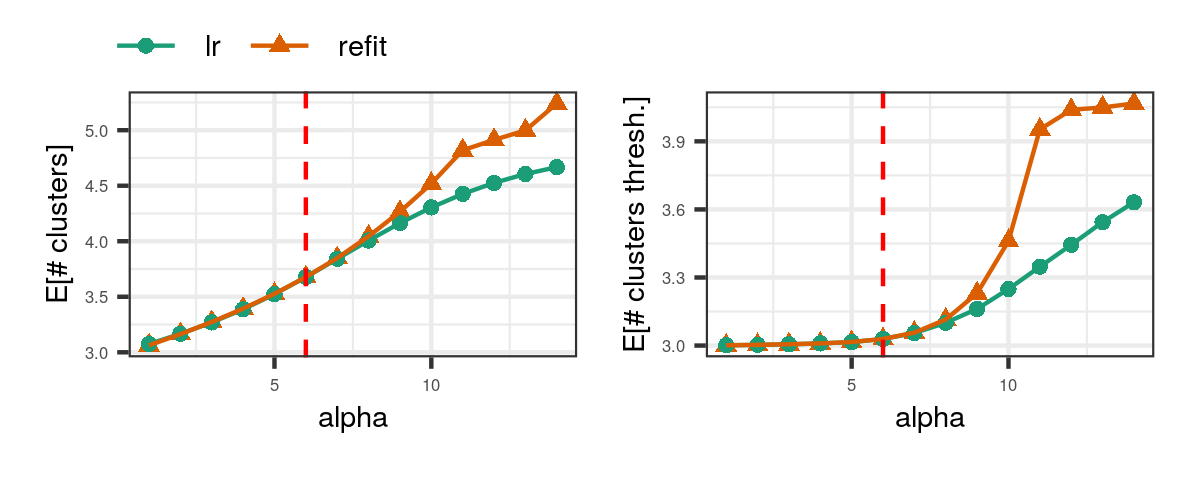
\includegraphics[width=0.980\linewidth,height=0.392\linewidth]{figure/iris_alpha_sens-1} 

}

\caption[The expected number of clusters as $\alpha$ varies in the 
the BNP-GMM fit of the iris data]{The expected number of clusters as $\alpha$ varies in the 
the BNP-GMM fit of the iris data. 
On the left is the sensitivity of the in-sample quantity.  
On the right is the the predictive quantity. 
We compute the linear approximation at $\alpha=6$ and
extrapolate the expected number of clusters using the
linear approximation (green).
We compare against the expected number of clusters obtained by refitting the model at each $\alpha$ (orange). }\label{fig:iris_alpha_sens}
\end{figure}


\end{knitrout}


% 
% - we demonstrate the utility of the influence function 
% - figure ref top three rows shows three different functional perturbations. 
% - can't really tell from densities how these will affect posterior statistic
% - but they do in fact have very different effects (in sign and size). 
% - but their effects make sense when looking at the influence function
% 
% -last row is worst-case

We next consider functional perturbations, 
and we demonstrate the ability of the influence function to 
provide guidance on the anticipated effect of perturbations 
on the posterior quantity. 
Each row of \figref{iris_fsens} presents a different 
multiplicative perturbation $\phi$ to the initial $\betadist{1, 6}$ stick distribution. 
The left column of \figref{iris_fsens} displays the perturbation $\phi$ overlayed with the prior-weighted influence function for $\gclusters$.
The perturbations are of the form 
$\log \phi(x) = e^{2(x - \mu)^2}$, with each perturbation having a 
different value of $\mu$. 
The middle column displays the initial density,
$p_0(\nu_k) = \betadist{\nu_k\vert 1, 6}$, along with the perturbed density,
$p_1(\nu_k) = \betadist{\nu_k\vert 1, 6}\phi(\nu_k)$.

Each perturbation $\phi$ produces distinct changes in the expected number of in-sample clusters $\gclusters$ (\figref{iris_fsens} right column). 
The changes in $\gclusters$ after each perturbation are 
different in both sign and magnitude. 
By examining the perturbed densities alone, it is difficult to anticipate 
the effect of the perturbation on $\gclusters$. 
However, the sign and magnitude of the change in $\gclusters$ is well-explained by the influence function. 
When $\log\phi$ is centered at a location where the influence function is negative, the effect on $\gclusters$ is negative (top row); 
conversely, when $\log\phi$ is centered at a location where the influence function is positive, the effect on $\gclusters$ is positive (bottom row); finally, when $\log\phi$ is centered at a location where the influence is both negative and positive, the effects cancel, and the change in the posterior statistic is roughly zero (middle row). 
In each case, the linear approximation is able to capture the changes in the posterior statistic. 
In applications below, we use influence function to guide our choice of functional perturbaton and to explain why some perturbations result in greater sensitivity than others. 

Finally, we consider the 
worst-case perturbation with unit $L_\infty$ norm.
Recall that the worst-case perturbation with unit $L_\infty$ norm is a 
step-function taking on values $\pm1$ corresponding 
to the sign of the influence function (\figref{iris_worstcase} left).  
The middle column of \figref{iris_worstcase} shows the prior density perturbed by the worst-case perturbation; 
the right column shows the effect on $\gclusters$. 
We see that this worst-case perturbation has a much larger effect on
$\gclusters$ compared to the other unit $L_\infty$ norm perturbations in
\figref{iris_fsens}. 
However, even with the worst-case perturbation, 
the change in $\gclusters$ is still small;
we thus conclude that in the iris dataset $\gclusters$ appears to be a quantity insensitive to the prior. 



\begin{knitrout}
\definecolor{shadecolor}{rgb}{0.969, 0.969, 0.969}\color{fgcolor}\begin{figure}[!h]

{\centering 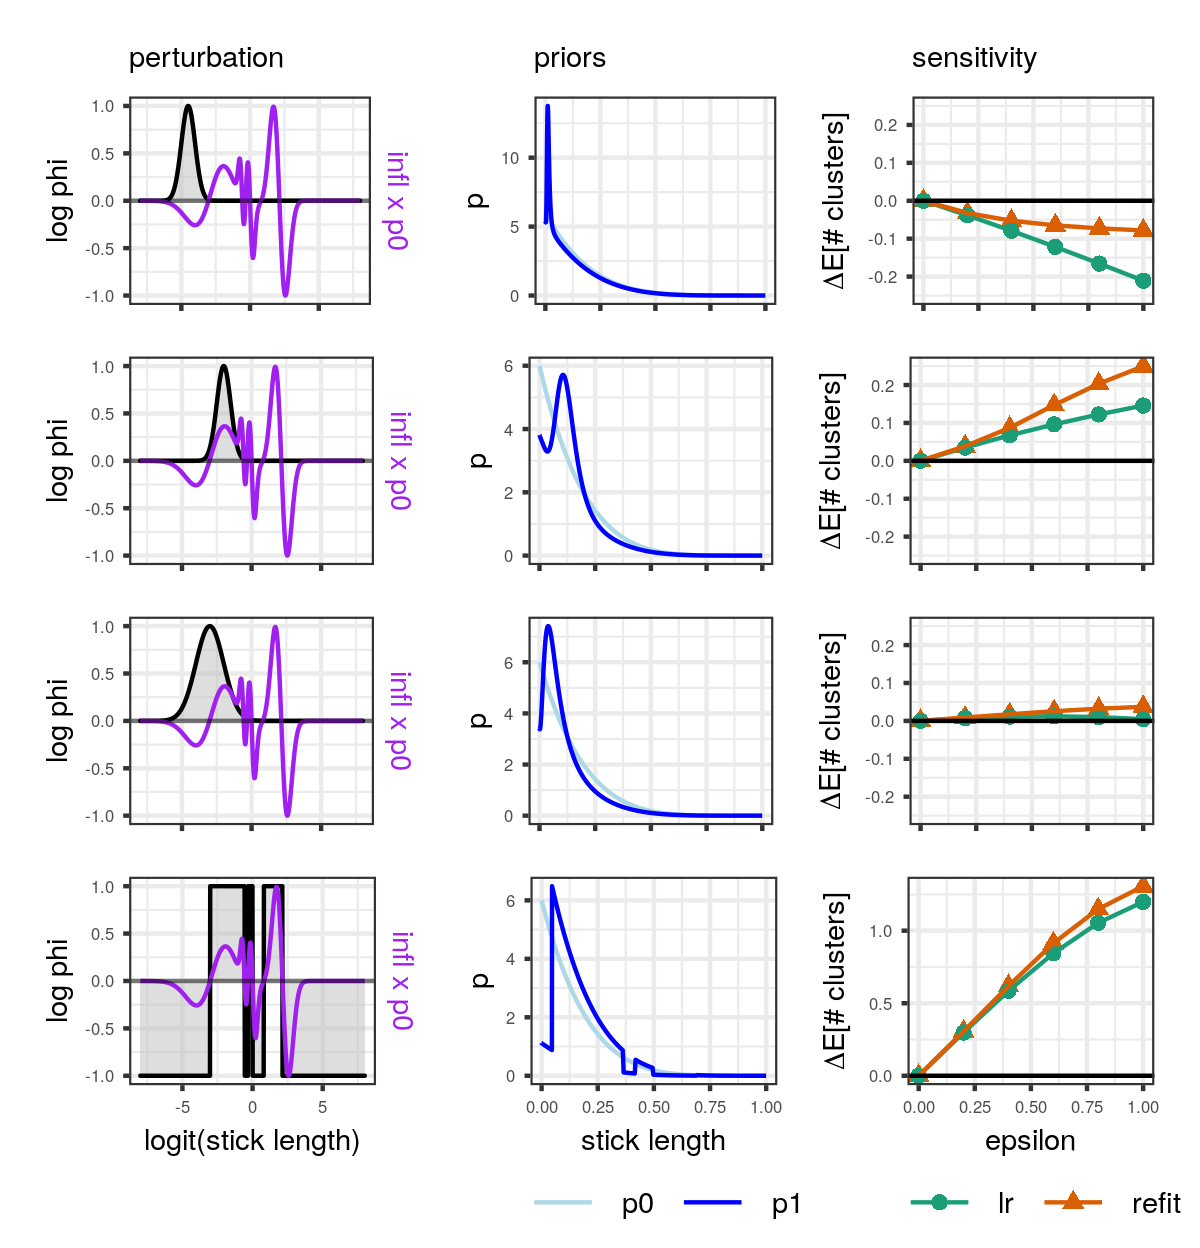
\includegraphics[width=0.980\linewidth,height=0.862\linewidth]{figure/iris_fsens-1} 

}

\caption{Sensitivity of
        the expected number of in-sample clusters in the iris dataset
        to three multiplicative perturbations with 
        unit $L_{\infty}$-norm 
        (Left) The log multiplicative perturbation $\log\phi$ in grey.        
        In purple is the prior-weighted influence function, scaled to also have 
        unit $L_{\infty}$-norm. 
        (Middle) The original prior density $p_0$ and 
        the perturbed prior density $p_1 = p_0\times \phi$. 
        (Right) The effect of the perturbation 
        on the change in expected number of clusters as a function of $\epsilon$. }\label{fig:iris_fsens}
\end{figure}


\end{knitrout}


\begin{knitrout}
\definecolor{shadecolor}{rgb}{0.969, 0.969, 0.969}\color{fgcolor}\begin{figure}[!h]

{\centering 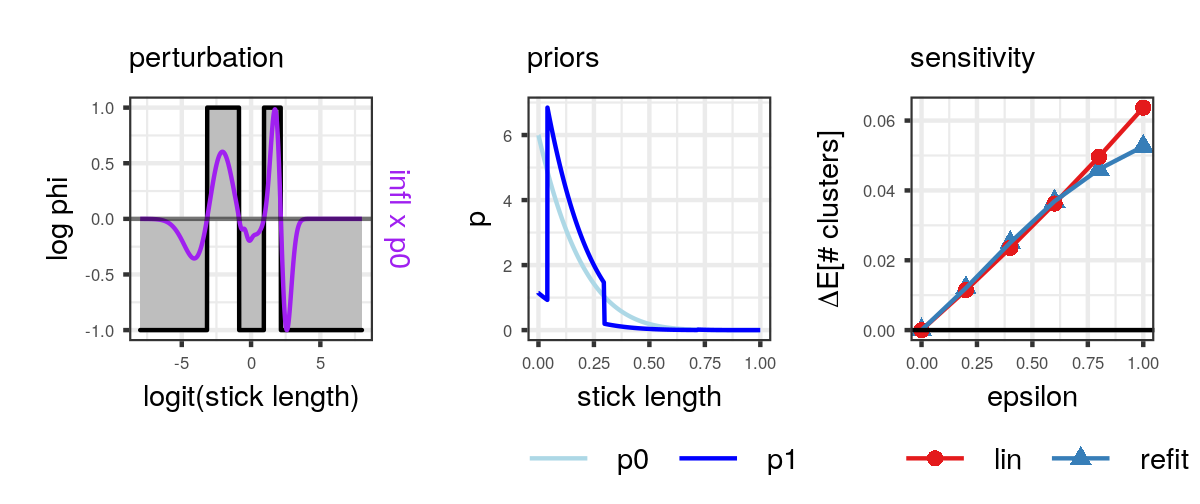
\includegraphics[width=0.980\linewidth,height=0.412\linewidth]{figure/iris_worstcase-1} 

}

\caption[Sensitivity of
        the expected number of in-sample clusters in the iris dataset
        to the worst-case multiplicative perturbations with 
        unit $L_{\infty}$-norm]{Sensitivity of
        the expected number of in-sample clusters in the iris dataset
        to the worst-case multiplicative perturbations with 
        unit $L_{\infty}$-norm.}\label{fig:iris_worstcase}
\end{figure}


\end{knitrout}

% \begin{table}[tb]
% \centering
% \caption{Compute time of results on the iris dataset. }
% \begin{tabular}{|r|r|}
%     \hline 
%     & time (seconds) \\ 
%     \hline 
%     Initial fit & sprintf('%1.2g', init_fit_time) \\
%     \hline 
%     Hessian solve for $\alpha$ sensitivity & 
%         sprintf('%1.2g', alpha_hess_time)\\
%     Linear approx. $\eta^{lin}(\alpha)$ for $\alpha = 1, ... , 16$ & 
%         sprintf('%1.2g', total_alpha_lr_time)\\
%     Refits $\eta(\alpha)$ for $\alpha = 1, ... , 16$ & 
%         sprintf('%1.2g', total_alpha_refit_time)\\
%     \hline 
%     The influence function & sprintf('%1.2g', infl_time)\\ 
%     Hessian solve for worst-case $\phi$ & 
%         sprintf('%1.2g', wc_hessian_time)\\
%     Linear approx. $\eta^{lin}(\epsilon)|_{\epsilon = 1}$
%     for worst-case $\phi$ & 
%         sprintf('%1.2g', wc_lr_time)\\
%     Refit $\eta(\epsilon)|_{\epsilon = 1}$ for worst-case $\phi$ & 
%         sprintf('%1.2g', wc_refit_time)\\ 
%     \hline 
% \end{tabular}
% \end{table}



\subsection{Regression mixture modeling}
%%%%%%%%%%%%%%%%%%%%%%%%%%%%%%%%%%%%%%
%%%%%%%%%%%%%%%%%%%%%%%%%%%%%%%%%%%%%%
% Do not edit the TeX file your work
% will be overwritten.  Edit the RnW
% file instead.
%%%%%%%%%%%%%%%%%%%%%%%%%%%%%%%%%%%%%%
%%%%%%%%%%%%%%%%%%%%%%%%%%%%%%%%%%%%%%



We consider the problem of clustering time-course gene expression data. 
While thousands of genes might be simultaneously 
measured in a given genomics experiment, 
many genes may exhibit similar expression patterns.  
Clustering gene expressions
is one way to reduce the dimensionality of a complex data set 
and to facilitate scientific interpretations of intricate biological processes. 
Often, such dimensionality reduction is used for exploratory analysis and
is a first step before further downstream investigation.  
It is important, therefore, to acertain the stability of the 
discovered clusters. 
 
We study a publicly available data set of mice gene expression
\citep{shoemaker:2015:ultrasensitive}.
Mice were infected with different influenza viruses, and expression levels of a set of genes were assessed at 14 time points after infection.
Our analysis focuses on mice treated with the ``A/California/04/2009'' strain. 
We normalize the data as described in
\citet{shoemaker:2015:ultrasensitive} and then apply the differential
analysis tool EDGE \citep{Storey:2005:significance} to rank the genes from most to least significantly differentially expressed. 
We fit a BNP model and run our analysis below on the top $\ngenes = 1000$ genes.

\subsubsection*{The model}

Each gene consists of $\ntimepoints = 42$ measurements of expression: three measurements (called biological replicates) at 14 unique timepoints.
The timepoints are unevenly spaced, with more frequent observations at the beginning. 
Following \citet{Luan:2003:clustering} we apply cubic B-splines to smooth the time course expression data. 
Specifically, we model the first 11 timepoints using
cubic B-splines with 7 degrees of freedom.
For the last three timepoints, $\timeindx = 72, 120, 168$ hours,
we use indicator functions. 
That is, if $\tilde \regmatrix$ is the design 
matrix where each column is a
B-spline basis vector evaluated at the $\ntimepoints$ measurement times, 
we append to $\tilde \regmatrix$ three additional columns: 
in these columns, entries are 1
if $\timeindx = 72, 120,$ or 168, repectively, and 0 otherwise. 
Call the full design matrix $\regmatrix$. 
We use indicators for the last three timepoints for numerical stability; 
without the indicator columns,
the matrix $\tilde \regmatrix^T \tilde \regmatrix$ is nearly singular
because the later timepoints are more spread out. 
See \figref{example_genes} for an example gene and the B-spline basis. 

%

\begin{knitrout}
\definecolor{shadecolor}{rgb}{0.969, 0.969, 0.969}\color{fgcolor}\begin{figure}[!h]

{\centering 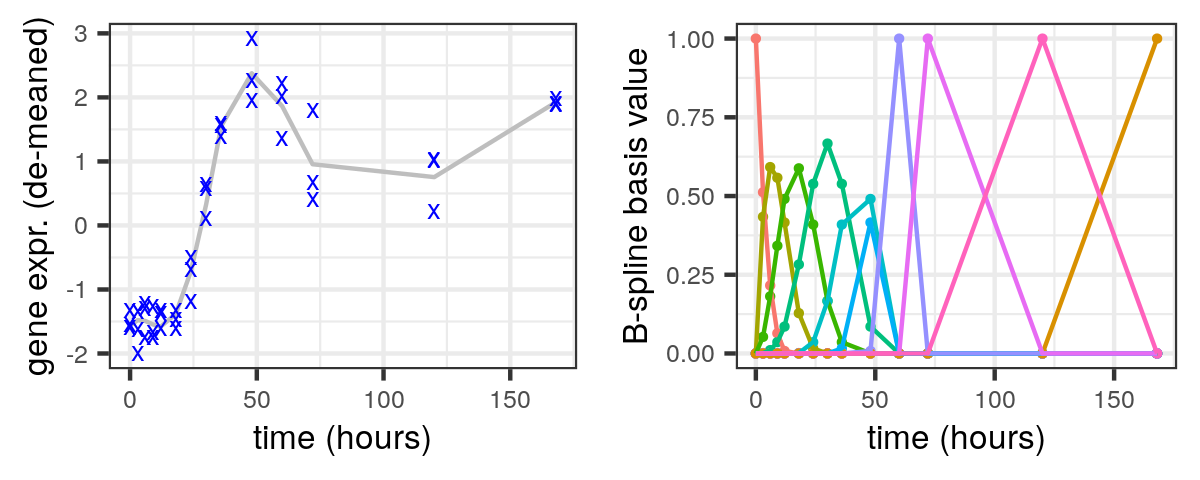
\includegraphics[width=0.980\linewidth,height=0.392\linewidth]{figure/example_genes-1} 

}

\caption[(Left) An example gene and its expression measured at 14 unique timepoints
    with three biological replicates at each timepoint.
     (Right) The cubic B-spline basis with 7 degrees of freedom, 
    along with three indicator functions for the last three timepoints, 
    $\timeindx = 72, 120, 168$]{(Left) An example gene and its expression measured at 14 unique timepoints
    with three biological replicates at each timepoint.
     (Right) The cubic B-spline basis with 7 degrees of freedom, 
    along with three indicator functions for the last three timepoints, 
    $\timeindx = 72, 120, 168$.}\label{fig:example_genes}
\end{figure}


\end{knitrout}
%


Let $\x_\n$ be the vector of observations for gene $\n$,
$(\x_{\n 1}, ..., \x_{\n \ntimepoints})^T$.
Each cluster is characterized by a vector of regression coefficients 
$\beta_k$ and a variance $\tau^{-1}_k$; 
the cluster parameters are $\theta_k = (\beta_k, \tau_k)$. 
The distribution of the data arising from cluster $k$ is 
\begin{align*}
\p(\x_\n | \theta_k, \b_{n}) = 
\normdist{\x_\n | \regmatrix\beta_k + \b_{n},
\tau_k^{-1}I_{\ntimepoints \times \ntimepoints}},
\end{align*}
where $\b_{n}$ is a gene-specific additive offset. 
We include the additive offset because we 
are interested in clustering the pattern of gene expression, 
not the absolute level. 

The joint distribution can be written in the same form as~\eqref{bnp_model}, 
except that the conditional log-likelihood also conditions on $b_n$, 
and we also include an additional prior term:
\begin{align*}
\MoveEqLeft
\logp(\x, \theta, \z, \nu) ={}
\nonumber\\&
    \sum_{n=1}^N \sum_{k=1}^{\kmax}
        \z_{\n\k} \left(
            \logp(\x_n \vert \theta_\k, \b_n) + \logp(\b_n) + \log \pi_\k
        \right) +
    \sum_{k=1}^{\kmax} \left(
        \log \pstick(\nuk) + \logp(\theta_\k)
    \right).
\end{align*}
We use a normal prior for the shifts $\b_n$, 
a multivariate normal prior for the coefficients $\beta_n$,
and a gamma prior for the inverse variance $\tau$. 

Our variational distribution factorizes as~\eqref{vb_mf}
with the addition
of a factor for the additive shift: 
\begin{align*}
\q(\zeta \vert \eta) =
    \left( \prod_{\k=1}^{\kmax - 1} \q(\nuk \vert \eta) \right)
    \left( \prod_{\k=1}^{\kmax} \q(\theta_\k \vert \eta) \right)
    \left( \prod_{\n=1}^{\N} \q(\z_{\n} \vert \eta) 
    \q(\b_{\n} \vert \z_{\n}, \eta)\right).
\end{align*}
Note that the variational distribution for $\b_\n$ conditions on $\z$.
We set $\q(\b_{\n} \vert \z_{\n} = k, \eta)$ to be Gaussian
with variational parameters dependent on $\k$. 
For simplicity in this application,
we let $\q(\theta_\k \vert \eta) = \delta (\theta_k \vert \eta)$, 
where $\delta(\cdot \vert \eta)$ denotes a point mass at a parameterized location. 

By parameterizing 
$\q(\z_{\n}, \b_{\n} \vert \eta) = \q(\z_{\n} \vert \eta)  \q(\b_{\n} \vert \z_{\n}, \eta)$ 
the optimal variational parameters for $\q(\z_{\n}, \b_{\n} \vert \eta)$ 
have a closed form given $\q(\nu, \theta \vert \eta)$. See \secref{put_in_appendix}. Therefore, our model fits the global/local framework as discussed in ... 
\todo{need to work on a section that talks about this}

We fitted the initial approximate posterior at $\alpha_0 = 6$. 
\figref{gene_centroids} shows the inferred smoothers 
$\regmatrix\mathbb{E}_\q[\beta_k]$ for selected clusters. 
\figref{gene_initial_coclustering} displays the inferred co-clustering matrix
$\coclusteringmatr(\eta)$, whose $(i,j)$-th entry is the
posterior probability that gene $i$ belongs to the same cluster
as gene $j$, given by 
\begin{align*}
\coclusteringmatr_{ij}(\eta) 
&= \expect{\q(\z\vert\eta)}{\ind{\z_{i} = \z_{j}}} \\
&= \sum_{k=1}^{\kmax}\left(\expect{\q(\z_i\vert\eta)}{\z_{ik}}
\expect{\q(\z_j\vert\eta)}{\z_{jk}}\right).
\end{align*}

Below, we evaluate the sensitivity of the inferred co-clustering matrix to 
both parametric and functional perturbations to the stick distribution. 


\begin{knitrout}
\definecolor{shadecolor}{rgb}{0.969, 0.969, 0.969}\color{fgcolor}\begin{figure}[!h]

{\centering 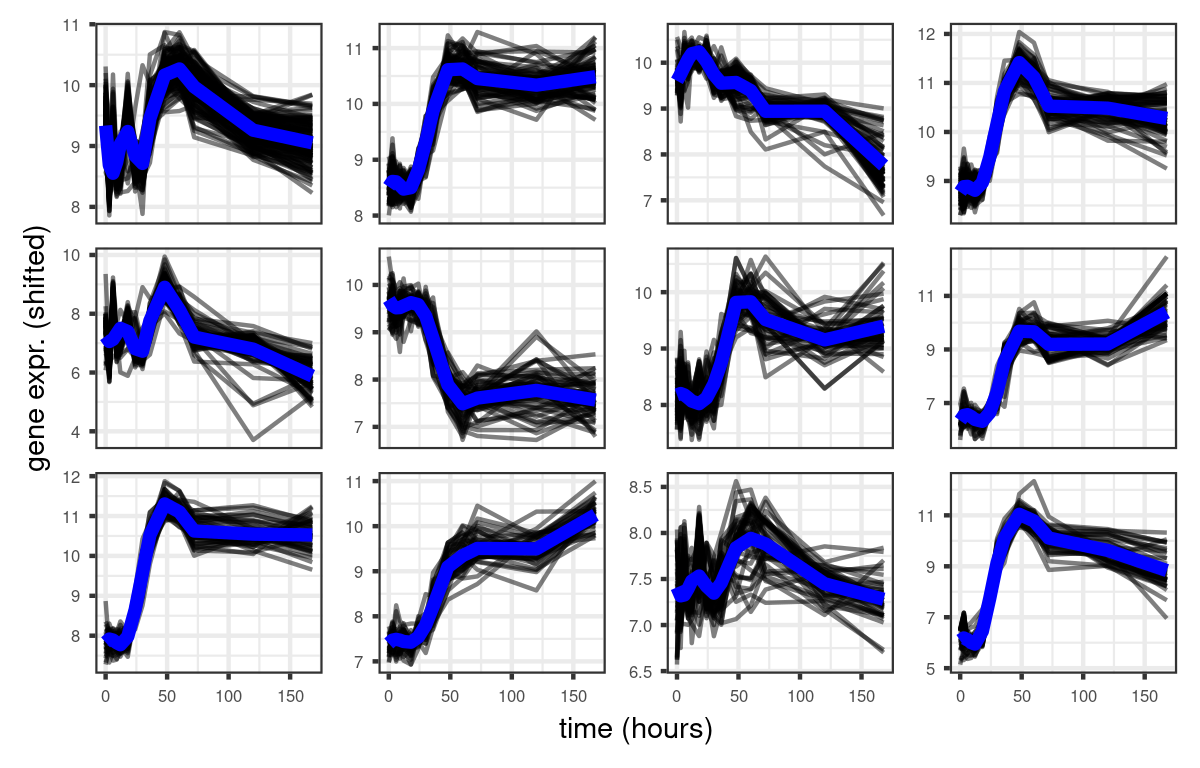
\includegraphics[width=0.980\linewidth,height=0.627\linewidth]{figure/gene_centroids-1} 

}

\caption[Inferred clusters in the mice gene expression dataset]{Inferred clusters in the mice gene expression dataset. 
    Shown are the twelve most occupied clusters. 
    In blue, the inferred cluster centroid. 
    In grey, gene expressions averaged over replicates and
    shifted by their inferred intercepts. }\label{fig:gene_centroids}
\end{figure}


\end{knitrout}



\begin{knitrout}
\definecolor{shadecolor}{rgb}{0.969, 0.969, 0.969}\color{fgcolor}\begin{figure}[!h]

{\centering 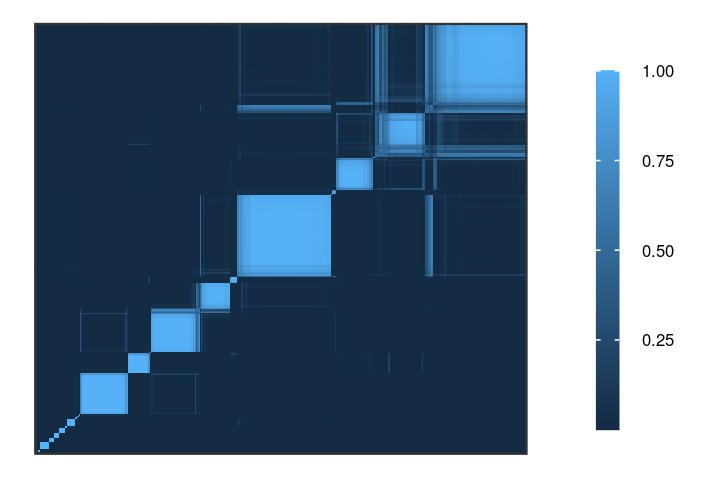
\includegraphics[width=0.588\linewidth,height=0.400\linewidth]{figure/gene_initial_coclustering-1} 

}

\caption[The inferred co-clustering matrix of gene expressions at $\alpha_0 = 6.$ ]{The inferred co-clustering matrix of gene expressions at $\alpha_0 = 6.$ }\label{fig:gene_initial_coclustering}
\end{figure}


\end{knitrout}


\subsubsection*{Sensitivity analysis}

We first evaluate the sensitivity of the co-clustering matrix $\coclusteringmatr$ 
to the choice of $\alpha$ in the
$\betadist{\nuk \vert 1, \alpha}$ stick distribution. 
Let $\coclusteringmatr_0 := \coclusteringmatr(\etaopt(\alpha_0))$ be the co-clustering matrix inferred at $\alpha_0$, 
and let $\Delta\coclusteringmatr(\eta) := 
\coclusteringmatr(\eta) - \coclusteringmatr_0$ be 
the difference in co-clustering matices after a change in the variational parameters $\eta$. 
We formed the linear approximation at $\alpha_0$ and computed
the change in co-clustering under the linearly approximated 
variational parameters, 
$\Delta\coclusteringmatr(\etalin(\alpha))$, at $\alpha = 1$ and $\alpha = 11$. 
For either $\alpha$, the change in the co-clustering matrix 
is miniscule (\figref{gene_alpha_coclustering}):
the largest entry of either matrix $\Delta\coclusteringmatr(\etalin(1))$ 
or $\Delta\coclusteringmatr(\etalin(11))$ is of order $10^{-2}$. 
Refitting the approximate posterior at $\alpha = 1$ and $\alpha = 11$ 
and computing $\Delta\coclusteringmatr(\etaopt(\alpha))$
confirms the insensitivity predicted by the linear approximation. 
Beyond capturing insensitivity, the linear approximation was also able to
approximate the sign and size of the changes in the individual entries of the coclustering matrix (these changes abeit small).  


\begin{knitrout}
\definecolor{shadecolor}{rgb}{0.969, 0.969, 0.969}\color{fgcolor}\begin{figure}[!h]

{\centering 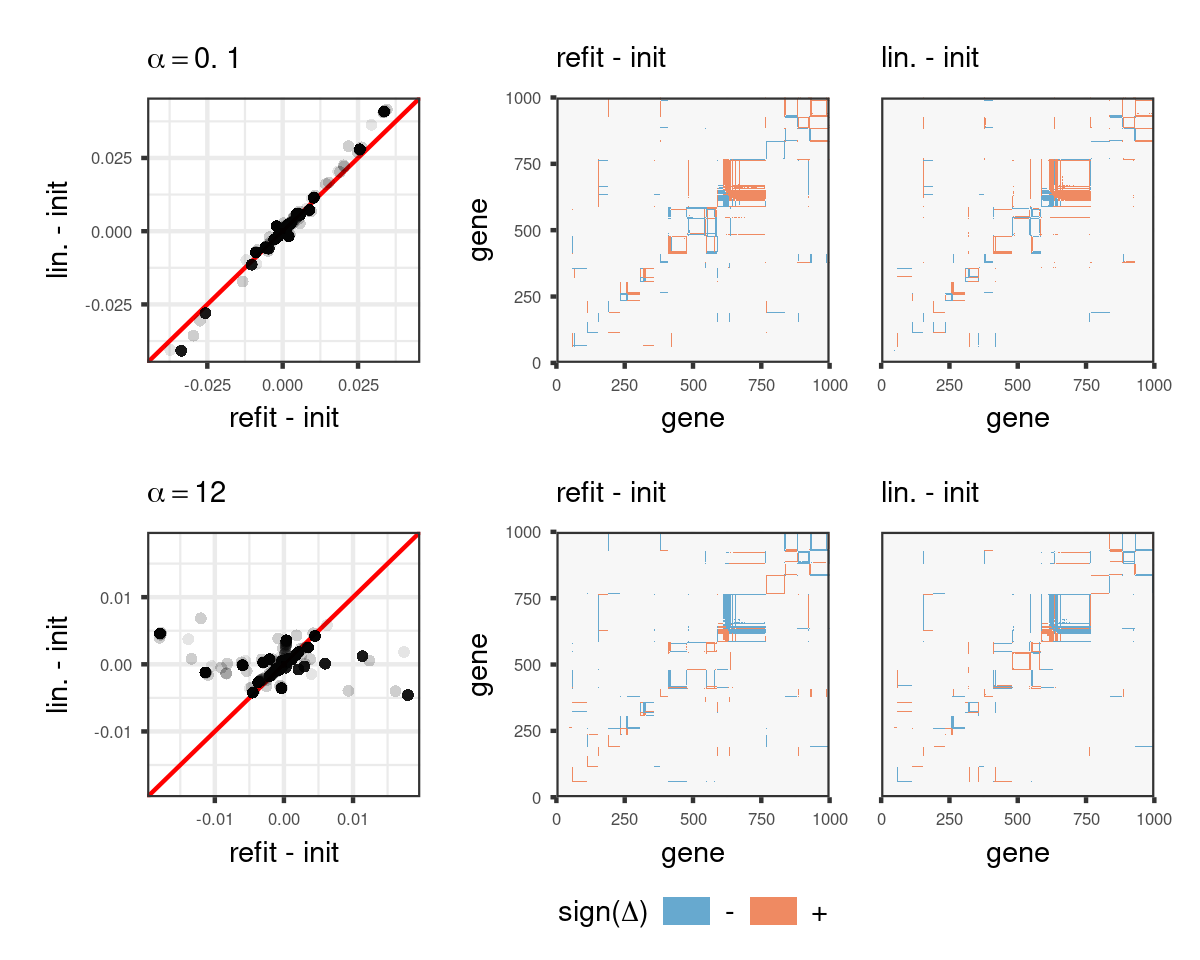
\includegraphics[width=0.980\linewidth,height=0.784\linewidth]{figure/gene_alpha_coclustering-1} 

}

\caption[Differences in the 
     co-clustering matrix at $\alpha = 1$ (top row)
     and $\alpha = 11$ (bottom row),
     relative to the co-clustering matrix at $\alpha_0 = 6$.
     We compare differences obtained with the linearly approximated 
     variational parameters against changes observed after 
     refiting]{Differences in the 
     co-clustering matrix at $\alpha = 1$ (top row)
     and $\alpha = 11$ (bottom row),
     relative to the co-clustering matrix at $\alpha_0 = 6$.
     We compare differences obtained with the linearly approximated 
     variational parameters against changes observed after 
     refiting. 
     (Left) a scatter plot of differences under the linear approximation 
     against differences after refitting, where
     each point represents an entry of the co-coclustering matrix.
     (Middle) the difference in co-clustering matrix observed after refitting. 
     (Right) the difference observed under the linearly approximated variational
     parameters. 
     For visualization, values in the heatmaps
     are clipped at $\pm 10^{-3}$. }\label{fig:gene_alpha_coclustering}
\end{figure}


\end{knitrout}


Insensitivity to $\alpha$ does not necessarily rule out insensitivity to other prior perturbations, however. 
As demonstrated in \secref{results_iris},
the influence function can provide guidance on which functional perturbations may result in greater sensitivity for a chosen posterior quantity. 
However, the co-clustering matrix as a posterior quantity is 
$\ngenes^2$-dimensional and 
thus does not lend itself to an easily interpretable influence function. 
We therefore summarize the co-clustering matrix into a scalar quantity: 
we use the sum of the eigenvalues of the symmetrically normalized graph Laplacian. 
This quantity has close connection with 
the number of distinct components in a graph CITE. 
Let this posterior quantity be denoted $\laplacianevsum$, given by 
\begin{align*}
  \laplacianevsum(\eta) = 
  \text{Tr}\left(
  I - D(\eta)^{-1/2} \coclusteringmatr(\eta) D(\eta)^{-1/2}
  \right),
\end{align*}
where $D(\eta)^{-1/2}$ is the diagonal matrix with entries $d_i = \sum_{j=1}^{\ngenes}[\coclusteringmatr(\eta)]_{ij}$. 
(And recall that the trace of a matrix is equivalent to the sum of its eigenvalues).

Because $\laplacianevsum(\eta)$ is a scalar quantity, we can plot its influence function. 
We choose a functional perturbation $\log\phi_{\textrm{ev}}$ that has a large, positive inner-product with the influence function.
In this case, we construct $\log\phi_{\textrm{ev}}$
using two Gaussian bumps aligned with
the two largest modes of the prior-weighted influence function
(\figref{gene_fpert_coclustering} top left). 
We anticipate $\log\phi_{\textrm{ev}}$
to have a large effect on $\laplacianevsum$. 
With $\laplacianevsum$ a proxy for our actual posterior quantity of interest, 
the full co-clustering matrix, we then expect that the co-clustering matrix 
will also experience large changes. 





Our intuition is confirmed in \figref{gene_fpert_coclustering}. 
After perturbing by $\log\phi_{\textrm{ev}}$, 
the largest changes in the co-clustering matrix are of now of order $10^{-1}$, 
compared with changes on the order of $10^{-2}$ after the $\alpha$ perturbations. 
The linear approximation again able to capture the qualitative changes in the co-clustering matrix after refitting at the perturbed prior. 


\begin{knitrout}
\definecolor{shadecolor}{rgb}{0.969, 0.969, 0.969}\color{fgcolor}\begin{figure}[!h]

{\centering 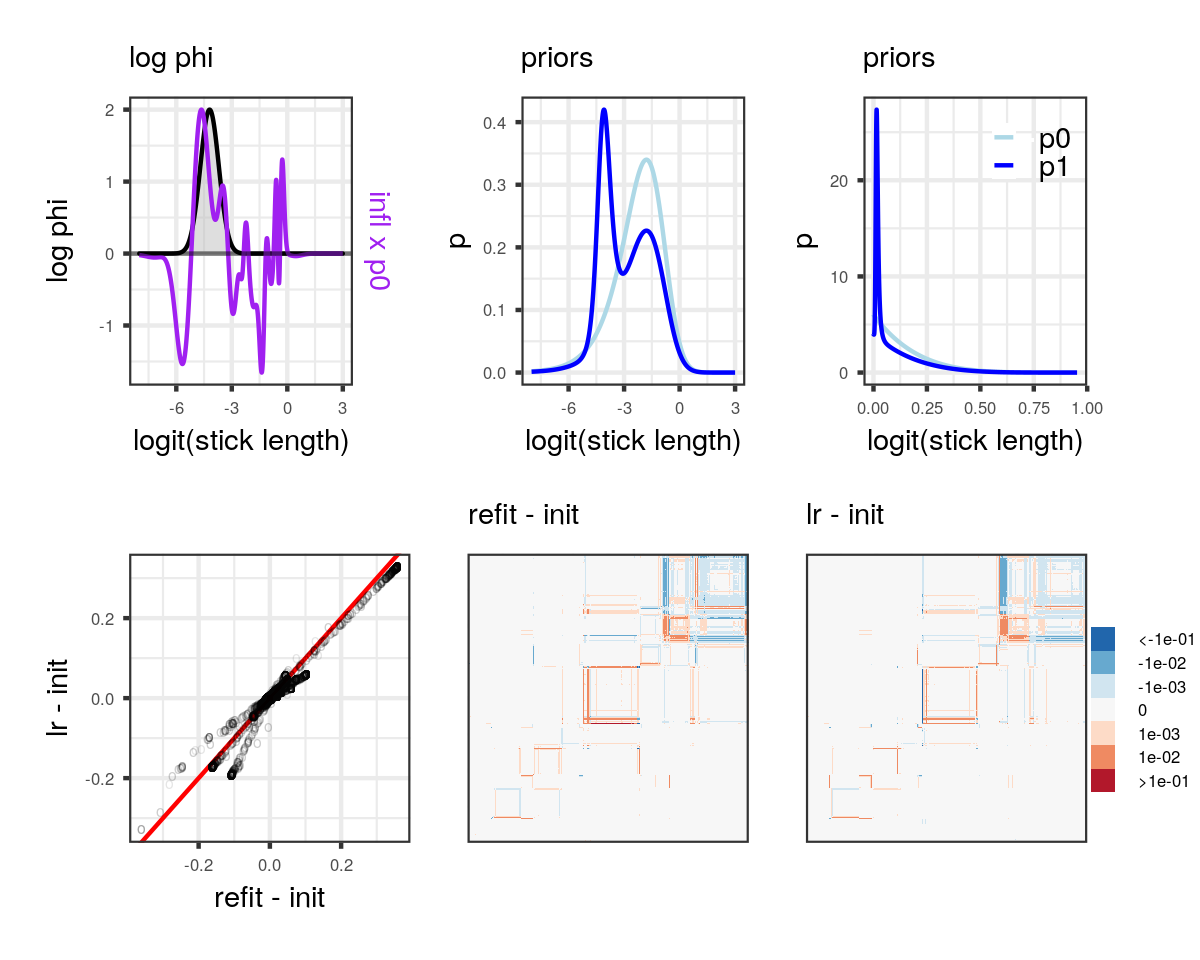
\includegraphics[width=0.980\linewidth,height=0.784\linewidth]{figure/gene_fpert_coclustering-1} 

}

\caption[Effect on the co-clustering matrix after a multiplicative functional
     perturbation.
     The perturbation $\phi$ (top left, in grey) 
     is a difference of two Gaussian bumps 
     scaled to have $L_\infty$ norm equal to two.
     $\phi$ is chosen such that the Gaussian bumps roughly align with the 
     two largest modes of the influence function (top left, purple]{Effect on the co-clustering matrix after a multiplicative functional
     perturbation.
     The perturbation $\phi$ (top left, in grey) 
     is a difference of two Gaussian bumps 
     scaled to have $L_\infty$ norm equal to two.
     $\phi$ is chosen such that the Gaussian bumps roughly align with the 
     two largest modes of the influence function (top left, purple; 
     the influence function is scaled to also have $L_\infty$ norm equal to two).
     The effect of this perturbation on the prior density in the top right. 
     The bottom row shows the effect of this perturbation on 
    the coclustering matrix.
    For visualization, the differences in the heatmap 
     are clipped at $\pm 10^{-1}$.}\label{fig:gene_fpert_coclustering}
\end{figure}


\end{knitrout}

The influence function is able to explain why the co-clustering matrix is 
insensitive to $\alpha$.
The functional perturbation
that corresponds to a change in $\alpha$ is
\begin{align*}
\log \phi_\alpha(\nu_\k) :=
\log\betadist{\nu_\k\vert 1, \alpha} -
\log\betadist{\nu_\k\vert 1, \alpha_0}.
\end{align*}
The function $\log\phi_\alpha(\nu_\k)$ is large when the influence function is small and vice-versa (\figref{alpha_pert_logphi}),
resulting in a small inner-product between the influence function
and $\log\phi_\alpha$. 
Thus, the linear approximation will predict small changes, and 
the refitted results confirms the linear approximation predictions. 


\begin{knitrout}
\definecolor{shadecolor}{rgb}{0.969, 0.969, 0.969}\color{fgcolor}\begin{figure}[!h]

{\centering 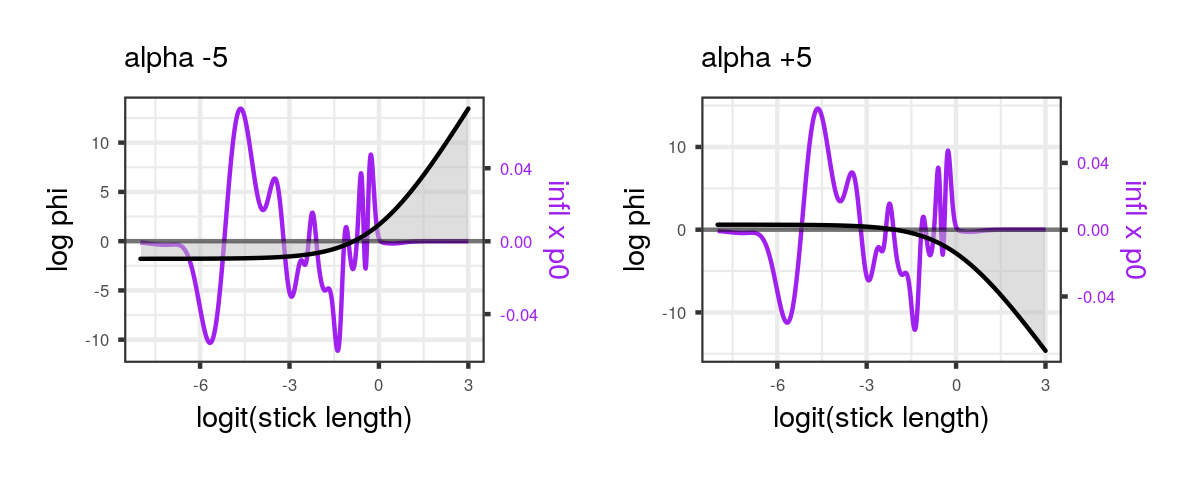
\includegraphics[width=0.882\linewidth,height=0.423\linewidth]{figure/alpha_pert_logphi-1} 

}

\caption[The multiplicative perturbations $\phi_\alpha(\cdot)$ that 
    corresponds to decreasing (left) or increasing (right) 
    the $\alpha$ parameter by five]{The multiplicative perturbations $\phi_\alpha(\cdot)$ that 
    corresponds to decreasing (left) or increasing (right) 
    the $\alpha$ parameter by five. }\label{fig:alpha_pert_logphi}
\end{figure}


\end{knitrout}

However, even with the selected functional perturbation,
the size of the differences in the co-clustering matrix remains modest. 
It is unlikely that any conclusions derived from the co-clustering matrix would have changed after the functional perturbation. 
The co-clustering matrix appears insensitive to perturbations in the stick-breaking distribution. 

Finally, we note that the computational cost of the linear approximation is again favorable compared with refitting (\tabref{mice_timing}). 
Forming the linear approximation, which requires a Hessian inversion, 
took 3-4 seconds; subsequent evaluations of $\etalin$ take milliseconds. 
Conversely, refitting the model after a prior perturbation can take up to 20 seconds. 

\begin{table}[tb]
\centering
\caption{Compute time of results on the mice data set. }
\tablabel{mice_timing}
\begin{tabular}{|r|r|}
    \hline 
    & time (seconds) \\ 
    \hline 
    Initial fit & 30 \\
    \hline 
    Hessian solve for $\alpha$ sensitivity & 
        3.9\\
    Linear approx. $\eta^{lin}(\alpha)$ for $\alpha = 1$ & 
        0.0013\\
    Linear approx. $\eta^{lin}(\alpha)$ for $\alpha = 11$ & 
        0.0012\\
    Refit $\eta(\alpha)$ for $\alpha = 1$ & 
        14\\
    Refit $\eta(\alpha)$ for $\alpha = 11$ & 
        13\\
    \hline
    The influence function & 4.3\\ 
    Hessian solve for $\phi$ perturbation &
        3.3\\
    Linear approx. $\eta^{lin}(\epsilon)$ at $\epsilon = 1$ &
        0.00099\\
    Refit $\eta(\epsilon)$ at $\epsilon = 1$ &
        22\\
    \hline
\end{tabular}
\end{table}


\subsection{Genetic admixture modeling with STRUCTURE}
%%%%%%%%%%%%%%%%%%%%%%%%%%%%%%%%%%%%%%
%%%%%%%%%%%%%%%%%%%%%%%%%%%%%%%%%%%%%%
% Do not edit the TeX file your work
% will be overwritten.  Edit the RnW
% file instead.
%%%%%%%%%%%%%%%%%%%%%%%%%%%%%%%%%%%%%%
%%%%%%%%%%%%%%%%%%%%%%%%%%%%%%%%%%%%%%



Our final data analysis example is an application of a Bayesian topic model to
population genetics. We consider a publicly available dataset from
\citet{galbusera:2000:thrush} that contains genotypes from 155 samples of an
endangered bird species, the Taita thrush. Individuals were collected from four
regions in southeast Kenya (Chawia, Mbololo, Ngangao, Yale), and each individual
was genotyped at seven micro-satellite loci. The four regions were once part of
a cohesive cloud forest that has since been fragmented by human development. For
this endangered bird species, understanding the degree to which populations have
grown genetically distinct is important for conservation efforts: well-separated
populations with little genetic diversity are particularly at risk of
extinction.  The goal of the analysis is to identify the presence of latent
populations, from which one can infer the population of origin for specific
loci, and estimate the degree to which populations are admixed in each
individual.


\subsubsection*{The model}

The data consists of consists of $\nindiv$ individuals genotyped at $\nloci$
loci. Let $\x_{\n\l\i}\in\{1, \ldots, J_\l\}$ be the observed genotype for
individual $\n$ at locus $\l$ and chromosome $\i$. $J_\l$ is the number of
possible genotypes at locus $\l$. For example, if the measurements are all
single nucleotides (A, T, C or G) then $J_\l = 4$ for all $\l$.

A latent population is characterized by the collection $\beta_k =
(\latentpop_{\k1}, \ldots, \latentpop_{\k\nloci})$ where
$\latentpop_{\k\l}\in\Delta^{J_\l - 1}$ are the latent frequencies for the $J_l$
possible genotypes at locus $\l$. Let $\z_{\n\l\i}$ be the assignment of
observation $\x_{\n\l\i}$ to a latent population. Notice that for a given
individual $\n$, different loci, or even different chromosomes at a given locus,
may have different population assignments. The distribution of
$\x_{\n\l\i}\in\{1, \ldots, J_\l\}$ arising from population $\k$ is
%
\begin{align*}
\p(\x_{\n\l\i} \vert \latentpop_{\k}) =
\categoricaldist{\x_{\n\l\i}\vert \latentpop_{\k\l}}.
\end{align*}

Unlike the previous models, we now have a stick-breaking process for each
individual. Draw sticks
%
\begin{align*}
\nu_{\n\k} \iid \pstick(\nu_{\n\k}) \quad \forall \n = 1, \ldots, \nindiv; \k = 1, 2, \ldots \infty.
\end{align*}
%
The prior assignment probability vector $\latentadmix_{\n} =
(\latentadmix_{\n1}, \latentadmix_{\n2}, \ldots)$, now unique to each
individual, is formed by the same stick-breaking construction as before,
%
\begin{align*}
\latentadmix_{\n\k} = \nu_{\n\k} \prod_{\k' < \k} (1 - \nu_{\n\k'}).
\end{align*}
%
The population assignment $\z_{\n\l\i}$ is drawn from the usual multinomial
distribution
%
\begin{align*}
p(\z_{\n\l\i} | \latentadmix_\n) = \prod_{k=1}^{\infty} \latentadmix_{\n\k}^{\z_{\n\l\i\k}}.
\end{align*}
%
In this genetics application, we call $\latentadmix_{\n}$ the \textit{admixture}
of individual $\n$.

This model is identical to fastSTRUCTURE, a model proposed in
\citet{pritchard:2000:structure, raj:2014:faststructure}, except that we replace
the Dirichlet prior in fastSTRUCTURE with an infinite stick-breaking process.
The result is a model similar to a hierarchical Dirichlet process for topic
modeling \citep{teh:2006:hdp}, but without the top-level Dirichlet process. In
addition, genotypes at genetic markers take the place of words in a document; in
lieu of inferring ``topics," we infer latent populations.

The variational approximation is mean-field as before, and all distributions are
conditionally conjugate except for the stick-breaking proportions, which remain
logit-normal. See \appref{app_structure} for further details.



\begin{knitrout}
\definecolor{shadecolor}{rgb}{0.969, 0.969, 0.969}\color{fgcolor}\begin{figure}[!h]

{\centering 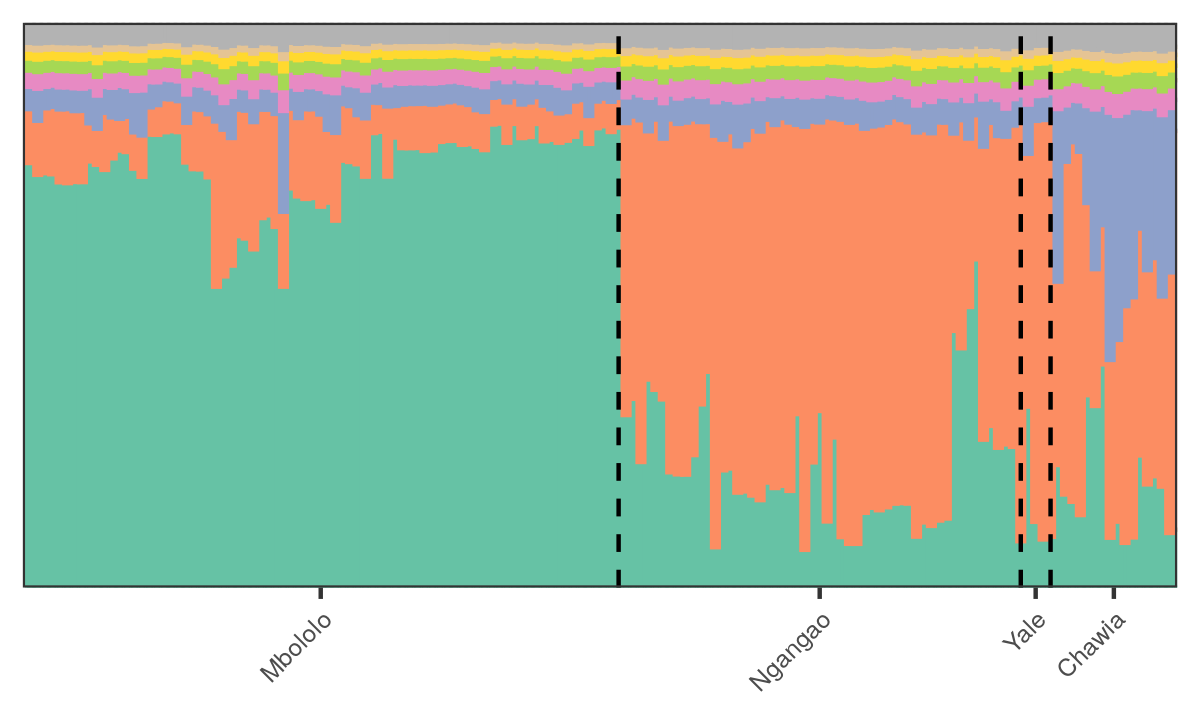
\includegraphics[width=0.980\linewidth,height=0.588\linewidth]{figure/stru_init_fit-1} 

}

\caption[The inferred individual admixtures at $\alpha_0 = 3$.
    Each vertical strip is an individual and each color
    a latent population.
    Lengths of colored segments represent the inferred admixture proportions.
    Individuals are ordered by the geographic region from which they were sampled
    (Mbololo, Ngangao, Yale, and Chawia).
    In the text, we refer to the green, orange, and purple latent populations
    as population 1, 2, and 3, respectively]{The inferred individual admixtures at $\alpha_0 = 3$.
    Each vertical strip is an individual and each color
    a latent population.
    Lengths of colored segments represent the inferred admixture proportions.
    Individuals are ordered by the geographic region from which they were sampled
    (Mbololo, Ngangao, Yale, and Chawia).
    In the text, we refer to the green, orange, and purple latent populations
    as population 1, 2, and 3, respectively. }\label{fig:stru_init_fit}
\end{figure}


\end{knitrout}

\subsubsection*{Quantity of interest}

The posterior quantities of interest in this application
are the individual admixtures $\pi_\n$.
\figref{stru_init_fit} plots the inferred admixtures $\pi_\n$ for all
individuals $\n$ under a $\gem$ prior with parameter $\alpha_0 = 3$.
The choice of $\alpha_0 = 3$ corresponds to roughly four distinct populations {\em a priori}, motivated by the fact that the individuals come from four geographic regions.
We will examine the robustness of the inferred admixtures to the prior below.

In the posterior at $\alpha_0$, there
appear to be three dominant latent populations, which we arbitrarily label as
populations 1, 2, and 3 (\figref{stru_init_fit}).
The inferred admixture proportions generally correspond with the geographic regions from which each individuals are sampled.

Notably, outlying admixtures among individuals from the same geographic region provide clues into the historical migration patterns of this species.
For example,
while individuals collected from the Mbololo region are inferred to be admixed
primarily with population 1, several individuals from this region have
abnormally large admixture proportions of population 2. Conversely, while
individuals collected from the Ngangao region are admixed primarily with
population 2, a few of these individuals have abnormally large admixture
proportions of population 1. This suggests that some migration has occurred
between the Mbololo and Ngangao regions.

We evaluate the sensitivity of this conclusion to possible prior perturbations.
Consider the posterior statistic
%
\begin{align*}
\gadmix(\eta; \mathcal{N}, k) =
 \expect{\q(\pi\vert\eta)}{\frac{1}{|\mathcal{N}|}\sum_{n\in\mathcal{N}}
\pi_{\n\k}},
\end{align*}
%
the average admixture proportion of population $\k$ in a set of
individuals $\mathcal{N}$.

Below, we present results on three variations of $\gadmix$, corresponding to
indididuals hightlighted as ``A," ``B", or ``C" in the top row of \figref{stru_func_sens}:
$\mathcal{N} = \{26, ..., 31\}$ and $k = 2$,
corresponding to the six individuals from the Mbololo region with outlying proportions of population 2;
$\mathcal{N} = \{125, ..., 128\}$ and $k = 1$,
corresponding to the four individuals from the Ngangao region with outlying proportions of population 1;
$\mathcal{N} = \{139, ..., 155\}$ and $k = 3$,
corresponding to all individuals from the Chawia region.
The first two posterior quantities relate to the inferred migration between
the Mbololo and Ngangao regions.
In the last case, we are studying the robustness of having a third latent
population present, a population which primarily appears in Chawia individuals.

\subsubsection*{Functional sensitivity}

In \figref{stru_func_sens}, we construct the worst-case negative perturbation
for decreasing each of our three variant of $\gadmix$, in order to see
whether the biologically interesting patterns can be made to disappear
with different prior choices.

\todo{Make the text easier to match up with the picture, which doesn't
have the populations (Ngangao, etc) labeled.  Right now it's hard to see
what's going on.}

\todo{I think this whole section could be easier to understand and much more
compact.  Basically just say that A is non-robust, B is robust, and on C
the linear approximation and refit disagree.  Then we investigate A more.}

Under the
linearized variational parameters $\etalinglobal(\t)$, the admixture proportion
of population 2 in the outlying Mbololo individuals is nearly halved.
The same quantity computed after refitting the model confirms the
sensitivity predicted by the linearized variational parameters.

 On the other
hand, the presence of population 1 in the outlying Ngangao individuals appears
to be insensitive even after this worst-case perturbation. The linearized and
the refitted variational parameters again agree on this conclusion. Finally, the
presence of population 3 in the Chawia individuals is anticipated to be
sensitive by the linearized parameters, as this admixture proportion steadily
decreases as $t\rightarrow 1$. However, under the refits, this admixture
proportion does not decrease steadily but rather levels off after $t = 0.5$.



\begin{knitrout}
\definecolor{shadecolor}{rgb}{0.969, 0.969, 0.969}\color{fgcolor}\begin{figure}[!h]

{\centering 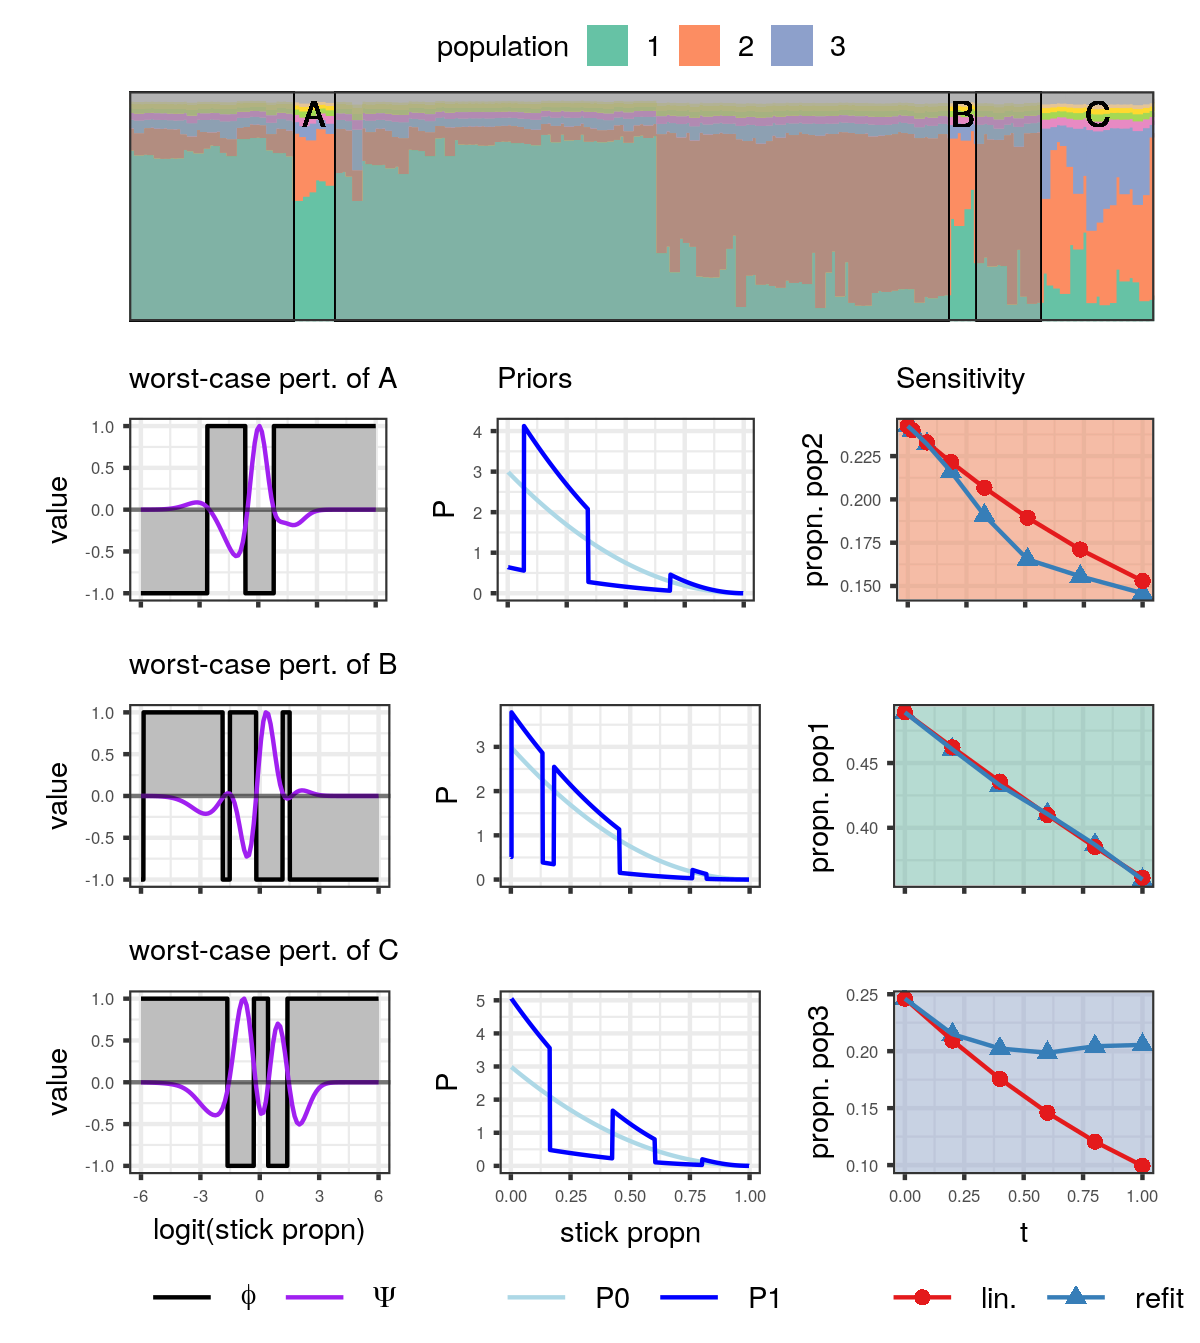
\includegraphics[width=0.980\linewidth,height=1.098\linewidth]{figure/stru_func_sens-1} 

}

\caption[Sensitivity of inferred admixtures for several outlying individuals.
     For individuals A,
     we examine the sensitivity of the admixture proportion of population 2.
     For individuals B,
     we examine the population 1 admixture
     For the individuals C, we examine the population 3 admixture.
     (Left column) The worst-case negative perturbation with
     $\norminf{\phi} = 1$
     in grey,
     plotted against the influence function in purple
     (scaled such that $\norminf{\psi} = 1$).
    (Middle column) The effect of the perturbation on the prior density.
    (Right column) Effects on the inferred admixture]{Sensitivity of inferred admixtures for several outlying individuals.
     For individuals A,
     we examine the sensitivity of the admixture proportion of population 2.
     For individuals B,
     we examine the population 1 admixture
     For the individuals C, we examine the population 3 admixture.
     (Left column) The worst-case negative perturbation with
     $\norminf{\phi} = 1$
     in grey,
     plotted against the influence function in purple
     (scaled such that $\norminf{\psi} = 1$).
    (Middle column) The effect of the perturbation on the prior density.
    (Right column) Effects on the inferred admixture. }\label{fig:stru_func_sens}
\end{figure}


\end{knitrout}


\todo{Say something about the fact that these priors are maybe too
adversarial.}


The conclusions from the linear approximation did not
perfectly agree with the conclusions from refitting variational approximation
in this data set and model.
For example, the admixture proportion of population 3 in individuals ``C" were predicted to be non-robust by our linear approximation but are in actuality are robust after refitting (bottom row \figref{stru_func_sens}).

Moreover, even though the linearized parameters
agreed with the refits in producing the diminished
overall admixture proportion of population 2 in individuals ``A"
(\figref{stru_func_sens} second row),
the approximation does does not perform uniformly well over all individual admixtures.
\figref{stru_func_sens_admix} plots the individual admixtures after the worst-case prior perturbation computed under both our linear approximation and after refitting.
The admixture proportion of population 2 in individual $n = 25$
dramatically increased after refitting with the perturbed prior $\p_1$;
the linearized parameters failed to reproduce this change.
For a more in depth discussion of the limitations of the linear approximation,
see \appref{app_structure_results}.

\todo{need to highlight main takeaway: even though linear approx works less well, still can use influence function to guide where to refit. }


\begin{knitrout}
\definecolor{shadecolor}{rgb}{0.969, 0.969, 0.969}\color{fgcolor}\begin{figure}[!h]

{\centering 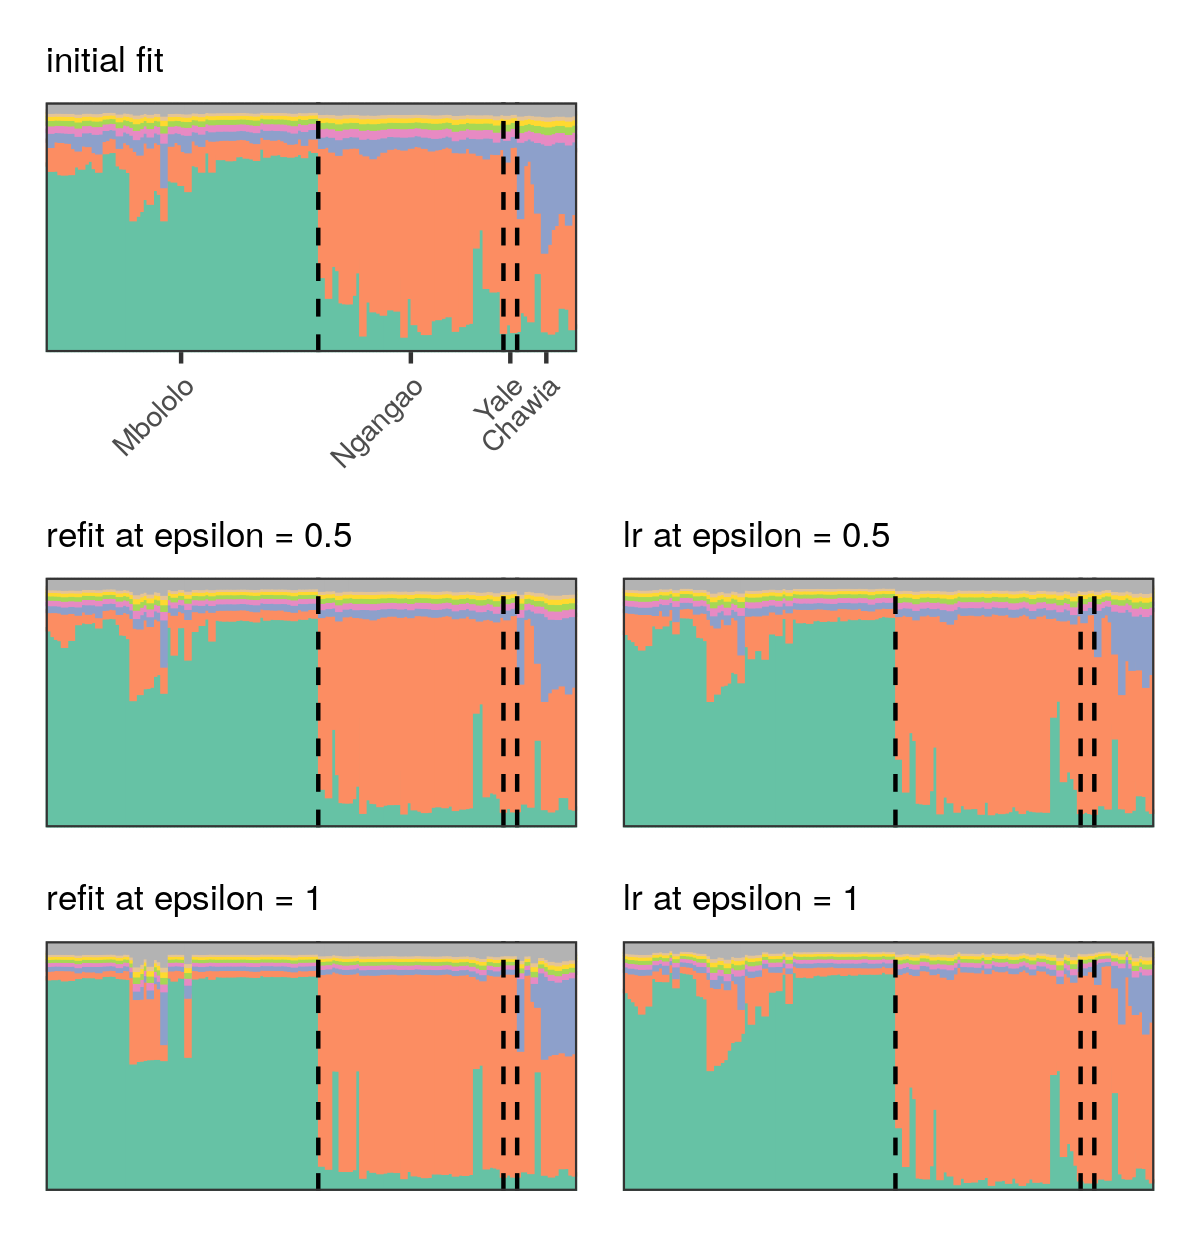
\includegraphics[width=0.980\linewidth,height=0.392\linewidth]{figure/stru_func_sens_admix-1} 

}

\caption{Inferred admixtures after the worst-case perturbation
     to individuals ``A" (see Figure~\ref{fig:stru_func_sens} for perturbation). }\label{fig:stru_func_sens_admix}
\end{figure}


\end{knitrout}


\newcommand{\StructureLimitationsA}{

\begin{knitrout}
\definecolor{shadecolor}{rgb}{0.969, 0.969, 0.969}\color{fgcolor}\begin{figure}[!h]

{\centering 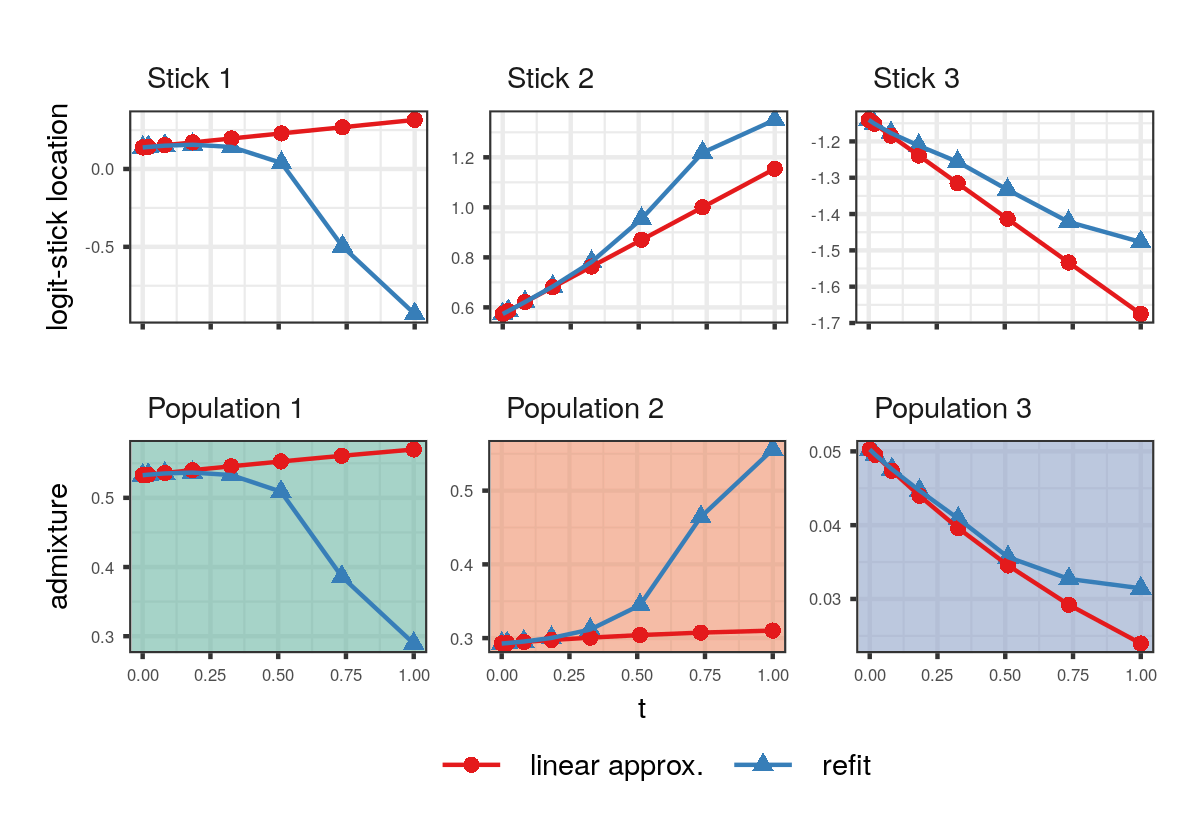
\includegraphics[width=0.980\linewidth,height=0.666\linewidth]{figure/stru_lin_bad_example-1} 

}

\caption[An individual $(\n = 26)$ for which
    the linearly approximated variational parameters
    poorly captured the
    change in admixture observed after refitting
    as $\t \rightarrow 1$.
    (Top row) the change in location parameter of the normally
    distributed logit-sticks, for the first three sticks.
    The response here is a variational parameter, so
    the approximation (red) is necessarily linear with respect to $\t$.
    (Bottom row) the change in the inferred admixtures for
    populations 1, 2, and 3]{An individual $(\n = 26)$ for which
    the linearly approximated variational parameters
    poorly captured the
    change in admixture observed after refitting
    as $\t \rightarrow 1$.
    (Top row) the change in location parameter of the normally
    distributed logit-sticks, for the first three sticks.
    The response here is a variational parameter, so
    the approximation (red) is necessarily linear with respect to $\t$.
    (Bottom row) the change in the inferred admixtures for
    populations 1, 2, and 3. }\label{fig:stru_lin_bad_example}
\end{figure}


\end{knitrout}
}

\newcommand{\StructureLimitationsB}{

\begin{knitrout}
\definecolor{shadecolor}{rgb}{0.969, 0.969, 0.969}\color{fgcolor}\begin{figure}[!h]

{\centering 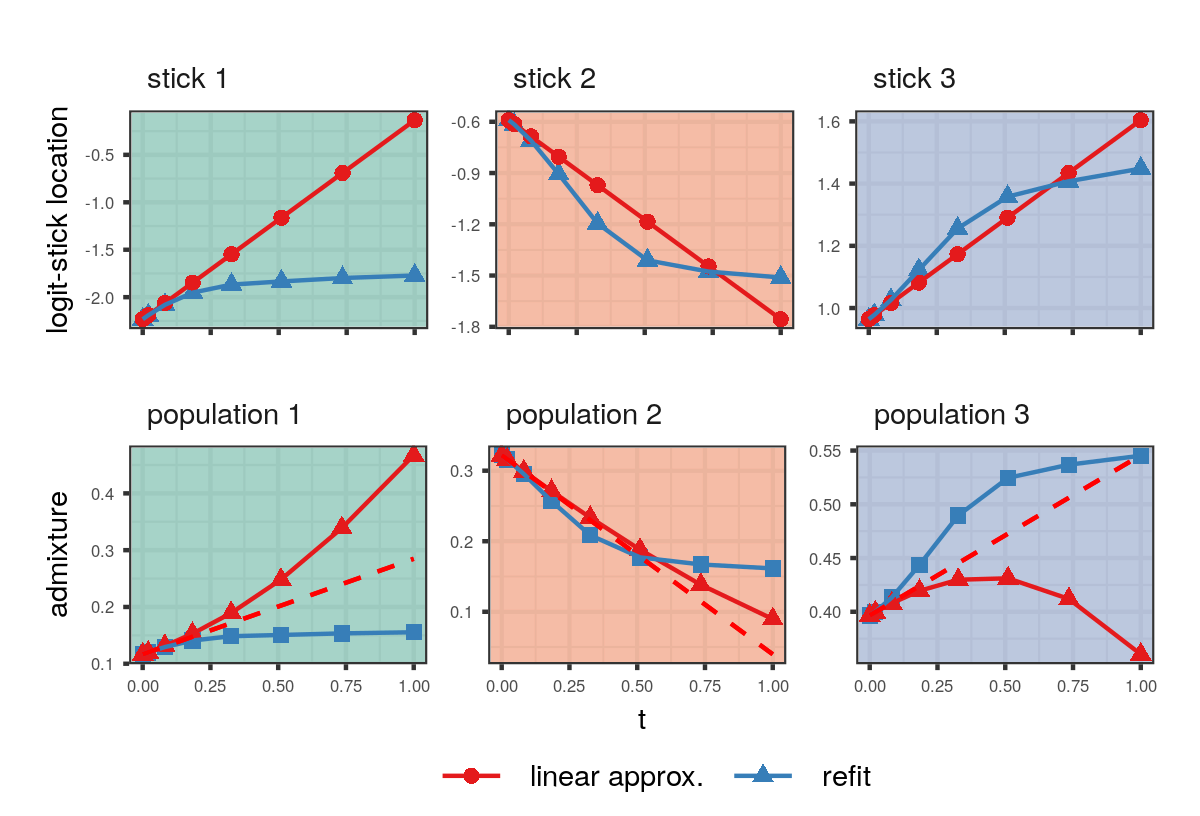
\includegraphics[width=0.980\linewidth,height=0.666\linewidth]{figure/stru_fully_lin_example-1} 

}

\caption[An example where
    linearizing the posterior quantity itself outperforms
    linearizing the variational parameters only.
    Shown are logit-stick location parameters (top row) and
    inferred admixtures (bottom row)
    for individual $n = 74$ and populations $k = 1, 2$ and $3$.
    Dashed red is the approximation $\glin(\t)$ formed by linearizing the
    inferred admixture $\expect{\q}{\pi_{\n\k}}$ with respect to prior
    parameter $t$.
    On the admixture proportion of population 3,
    $\glin(\t)$ outperforms $\g(\etalin(\t))$ (solid red)]{An example where
    linearizing the posterior quantity itself outperforms
    linearizing the variational parameters only.
    Shown are logit-stick location parameters (top row) and
    inferred admixtures (bottom row)
    for individual $n = 74$ and populations $k = 1, 2$ and $3$.
    Dashed red is the approximation $\glin(\t)$ formed by linearizing the
    inferred admixture $\expect{\q}{\pi_{\n\k}}$ with respect to prior
    parameter $t$.
    On the admixture proportion of population 3,
    $\glin(\t)$ outperforms $\g(\etalin(\t))$ (solid red). }\label{fig:stru_fully_lin_example}
\end{figure}


\end{knitrout}
}


\section{Conclusion}
This concludes.


\section{Acknowledgements}
Thanks to everyone.

% Manual newpage inserted to improve layout of sample file - not
% needed in general before appendices/bibliography.

\bibliography{references}
\bibliographystyle{plainnat}


\newpage

\appendix
\section*{Appendix A.}
\label{app:theorem}

Supplemental results

\end{document}
